\documentclass[11pt,a4paper]{article}
\usepackage[a4paper,left=1in,right=1in,top=1in,bottom=1in,headheight=14pt]{geometry}
\usepackage{microtype}
\usepackage{graphicx}
\usepackage{booktabs,tabularx,array,longtable}
\usepackage{xcolor}
\usepackage{tikz}
\usetikzlibrary{arrows.meta,positioning,automata,calc,fit,shapes.geometric}
\usepackage{listings}
\usepackage{fancyhdr}
\usepackage[font=small,labelfont=bf]{caption}
\usepackage{enumitem}
\usepackage{float}
\usepackage{setspace}
\usepackage[hidelinks]{hyperref}

\setlength{\parindent}{0pt}
\setlength{\parskip}{6pt}
\setstretch{1.15}
\sloppy

\definecolor{ink}{HTML}{1F2937}
\definecolor{mut}{HTML}{6B7280}
\definecolor{box}{HTML}{E8EEF7}
\definecolor{kw}{HTML}{1D4ED8}
\definecolor{cm}{HTML}{047857}

\lstdefinelanguage{VerilogX}[]{Verilog}{morekeywords={localparam,integer,initial,task,endtask}}
\lstset{
  language=VerilogX, basicstyle=\ttfamily\scriptsize, keywordstyle=\color{kw}\bfseries,
  commentstyle=\color{cm}, numbers=left, numberstyle=\tiny\color{mut}, numbersep=6pt,
  frame=single, rulecolor=\color{mut}, breaklines=true, columns=fullflexible,
  keepspaces=true, showstringspaces=false, tabsize=4, xleftmargin=14pt
}

\pagestyle{fancy}
\fancyhf{}
\fancyhead[L]{\small MOSART Training: Project 8}
\fancyhead[R]{\small Programmable Memory Controller}
\fancyfoot[L]{\small Shaun Praneeth Raj}
\fancyfoot[R]{\small Page \thepage}
\renewcommand{\headrulewidth}{0.4pt}

\newcommand{\sig}[1]{\texttt{#1}}

\begin{document}

%======================== TITLE PAGE ========================
\begin{titlepage}
\centering
\vspace*{1.2cm}
{\Large\bfseries MOSART TRAINING\par}
\vspace{0.3cm}
{\large Digital Design and RTL Project\par}
\vspace{2.2cm}
{\large Project 8\par}
\vspace{0.3cm}
{\LARGE\bfseries Programmable Memory Controller\par}
\vspace{0.5cm}
{\large RTL Design, Functional Verification and Synthesis\par}
\vspace{2.5cm}
\begin{tabular}{rl}
\textbf{Submitted by} & Shaun Praneeth Raj \\
\textbf{Programme} & B.Tech, Electronics and Communication Engineering \\
\textbf{Institution} & Anurag University, Hyderabad \\
\textbf{Target Device} & Xilinx Artix-7 (xc7a35tcpg236-1) \\
\textbf{Date} & 26 September 2026 \\
\end{tabular}
\vfill

\end{titlepage}

%======================== ABSTRACT ========================
\section*{Abstract}
\addcontentsline{toc}{section}{Abstract}
This report presents the design, verification and synthesis of a programmable synchronous memory controller for a small on-chip memory. The controller gives another digital block a simple request interface (\sig{read\_enable}, \sig{write\_enable}, \sig{address}, \sig{write\_data}) and returns \sig{read\_data} together with \sig{busy} and \sig{ready} status. A six-state Moore machine (IDLE, READ, WRITE, WAIT, DONE, ERROR) sequences each access, drives the memory strobes and inserts a run-time programmable number of wait states. A small configuration register bank allows the controller to be enabled or disabled, write protected, limited to a programmable address window, and interrogated through a sticky status register. Invalid requests (simultaneous read and write, out-of-range address, write under protection, request while busy) are rejected without touching memory and are recorded in the status register.

The design is written in synthesizable Verilog-2005 and is fully synchronous with a single clock and a synchronous active-high reset. A self-checking testbench with a behavioural reference model runs ten test groups, including a 500-access constrained-random regression, and completes 3356 checks with zero errors. Synthesis for the Xilinx 7-series fabric maps the design to 59 LUTs, one distributed RAM primitive (RAM32M) and 44 flip-flops, with a worst register-to-register path of six logic levels.

\newpage
\tableofcontents
\listoffigures
\listoftables
\newpage

%======================== 1 PROBLEM STATEMENT ========================
\section{Problem Statement}
Design and implement a programmable synchronous memory controller for a small on-chip memory. The controller shall provide a simple request interface that allows another digital block to perform memory read and write operations. It shall accept read and write requests, generate the memory control signals, return read data, report BUSY and READY status, and handle invalid or simultaneous read and write requests appropriately. The memory may be implemented as a register array, and a suitable controller may be built around an FSM containing IDLE, READ, WRITE, WAIT and DONE states.

The project follows the complete digital design flow: architecture definition, RTL design, functional verification by simulation, and synthesis with analysis of LUT usage, flip-flop usage and timing.

%======================== 2 REQUIREMENTS ========================
\section{Requirements and Specifications}

\subsection{System Requirements}
\begin{table}[H]
\centering
\caption{Functional requirements and how the design meets them}
\label{tab:req}
\small
\begin{tabularx}{\textwidth}{@{}l X X@{}}
\toprule
\textbf{ID} & \textbf{Requirement} & \textbf{Implementation} \\
\midrule
R1 & Accept read requests & \sig{read\_enable} sampled in IDLE; FSM enters READ \\
R2 & Accept write requests & \sig{write\_enable} sampled in IDLE; FSM enters WRITE \\
R3 & Generate memory control signals & \sig{mem\_re}, \sig{mem\_we}, \sig{mem\_addr}, \sig{mem\_wdata} decoded from FSM state and request latch \\
R4 & Provide read data & Registered memory output drives \sig{read\_data}, valid when \sig{ready} is high and held until the next read \\
R5 & BUSY / READY status & \sig{busy} high in every non-IDLE state; \sig{ready} one-cycle completion pulse \\
R6 & Handle simultaneous read and write & Request rejected in the ERROR state, memory untouched, STATUS.COLL set \\
R7 & Handle invalid requests & Out-of-range address, write under protection and request while busy are rejected and flagged \\
R8 & Programmability & Enable, write protect, 0 to 7 wait states and address limit set at run time through the configuration port \\
R9 & Register-array memory & 16 $\times$ 8-bit array with synchronous write and registered read \\
\bottomrule
\end{tabularx}
\end{table}

\subsection{Functional Specification}
\begin{itemize}[leftmargin=*,itemsep=2pt]
\item Memory organisation: 16 words of 8 bits (parameters \sig{ADDR\_W}~=~4, \sig{DATA\_W}~=~8).
\item One transaction in flight at a time. A request is a single-cycle pulse on \sig{read\_enable} or \sig{write\_enable} issued while \sig{busy} is low.
\item Access latency: with $N$ programmed wait states, \sig{ready} is asserted $N+2$ clock cycles after the edge that samples the request. The controller returns to IDLE one cycle later, so the maximum rate is one access every $N+3$ cycles.
\item Request validation order in IDLE: collision (both enables high) first, then address range (\sig{address} $\geq$ LIMIT), then write protection. The first failing check sends the FSM to ERROR.
\item A rejected request completes in two cycles with \sig{ready} and \sig{error} high together for one cycle.
\item While EN~=~0 the controller ignores requests entirely: \sig{busy} and \sig{ready} stay low.
\end{itemize}

\subsection{Input and Output Signals}
\begin{table}[H]
\centering
\caption{Top-level port list of \texttt{mem\_ctrl\_top}}
\label{tab:io}
\small
\begin{tabularx}{\textwidth}{@{}l c c X@{}}
\toprule
\textbf{Signal} & \textbf{Dir} & \textbf{Width} & \textbf{Description} \\
\midrule
\sig{clk} & in & 1 & System clock, 100 MHz target \\
\sig{reset} & in & 1 & Synchronous reset, active high \\
\sig{read\_enable} & in & 1 & Read request (one-cycle pulse) \\
\sig{write\_enable} & in & 1 & Write request (one-cycle pulse) \\
\sig{address} & in & 4 & Word address of the request \\
\sig{write\_data} & in & 8 & Data to be written \\
\sig{read\_data} & out & 8 & Data returned by a read, valid with \sig{ready} \\
\sig{ready} & out & 1 & Transaction finished (one-cycle pulse) \\
\sig{busy} & out & 1 & Transaction in progress, new requests not accepted \\
\sig{error} & out & 1 & Request rejected (pulse coincident with \sig{ready}) \\
\sig{cfg\_we} & in & 1 & Configuration register write strobe \\
\sig{cfg\_addr} & in & 2 & Configuration register address \\
\sig{cfg\_wdata} & in & 8 & Configuration write data \\
\sig{cfg\_rdata} & out & 8 & Configuration read-back (combinational) \\
\bottomrule
\end{tabularx}
\end{table}

\subsection{Register Map}
\begin{table}[H]
\centering
\caption{Configuration and status register map}
\label{tab:regmap}
\small
\begin{tabularx}{\textwidth}{@{}c l c c c X@{}}
\toprule
\textbf{Addr} & \textbf{Name} & \textbf{Bits} & \textbf{Access} & \textbf{Reset} & \textbf{Function} \\
\midrule
0x0 & CTRL & [0] & RW & 1 & EN: controller enable \\
    &      & [1] & RW & 0 & WP: write protect, writes rejected \\
0x1 & WAIT & [2:0] & RW & 0 & Wait states inserted per access (0 to 7) \\
0x2 & LIMIT & [4:0] & RW & 16 & Number of valid words; values above 16 saturate to 16 \\
0x3 & STATUS & [0] & W1C & 0 & COLL: simultaneous read and write request \\
    &        & [1] & W1C & 0 & RANGE: address $\geq$ LIMIT \\
    &        & [2] & W1C & 0 & WPV: write attempted while WP = 1 \\
    &        & [3] & W1C & 0 & OVR: request dropped while busy \\
    &        & [4] & RO  & 0 & BUSY: live copy of \sig{busy} \\
\bottomrule
\end{tabularx}
\end{table}
W1C bits are cleared by writing 1 to them. If an error event and a clear occur in the same cycle, the event wins so that no error is lost.

\subsection{Clock and Reset Architecture}
The whole design sits in one clock domain driven by \sig{clk}; there are no derived or gated clocks and therefore no clock domain crossings. Reset is synchronous and active high, the style recommended for Xilinx 7-series flip-flops (FDRE/FDSE), because it keeps the reset in the data path and avoids asynchronous recovery and removal checks. Reset returns the FSM to IDLE and the configuration registers to their defaults. The memory array itself is deliberately not reset: this allows it to map onto distributed RAM, and a controller reset does not destroy stored data (verified in test T9).

\subsection{Interface Definition}
The host protocol is a simple valid/ready handshake with one outstanding request:
\begin{enumerate}[leftmargin=*,itemsep=2pt]
\item The host waits for \sig{busy} = 0, then drives \sig{address}, \sig{write\_data} and one enable for a single clock cycle.
\item The controller latches the request, raises \sig{busy} on the next cycle and ignores further requests (flagging them as OVR).
\item When \sig{ready} pulses, the transaction is complete. For a read, \sig{read\_data} is valid in that cycle and remains stable until the next read. If \sig{error} is also high the request was rejected and the STATUS register gives the reason.
\end{enumerate}

%======================== 3 ARCHITECTURE ========================
\section{Architecture and Block Diagram}
The controller is partitioned into a control path (the FSM), a configuration path (register bank) and a storage path (memory array), as shown in Figure~\ref{fig:block}. The host sees only the top-level ports; all memory strobes are internal.

\begin{figure}[H]
\centering
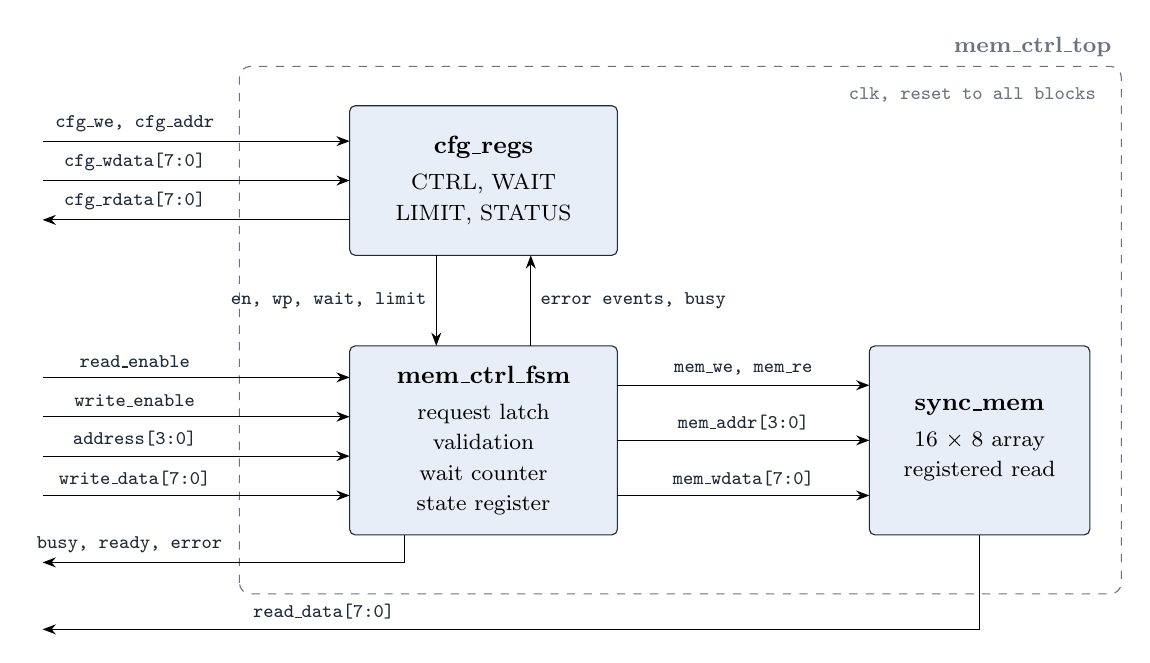
\begin{tikzpicture}[
  font=\small, >=Stealth,
  blk/.style={draw=ink, fill=box, rounded corners=2pt, minimum width=3.4cm, align=center, inner sep=6pt},
  lbl/.style={font=\scriptsize\ttfamily, color=ink}]
\node[blk, minimum height=2.4cm] (fsm) at (0,0) {\textbf{mem\_ctrl\_fsm}\\[2pt]\footnotesize request latch\\\footnotesize validation\\\footnotesize wait counter\\\footnotesize state register};
\node[blk, minimum height=1.9cm] (cfg) at (0,3.3) {\textbf{cfg\_regs}\\[2pt]\footnotesize CTRL, WAIT\\\footnotesize LIMIT, STATUS};
\node[blk, minimum height=2.4cm, minimum width=2.8cm] (mem) at (6.3,0) {\textbf{sync\_mem}\\[2pt]\footnotesize 16 $\times$ 8 array\\\footnotesize registered read};
\draw[mut, dashed, rounded corners=4pt] (-3.1,-1.95) rectangle (8.1,4.75);
\node[font=\footnotesize\bfseries, color=mut, anchor=south east] at (8.1,4.75) {mem\_ctrl\_top};
\node[lbl, color=mut, anchor=north east] at (7.9,4.6) {clk, reset to all blocks};
% host inputs
\foreach \y/\t in {0.8/read\_enable, 0.3/write\_enable, -0.2/address[3:0], -0.7/write\_data[7:0]}
  \draw[->] (-5.6,\y) -- node[lbl,above,pos=0.3]{\t} (-1.7,\y);
\draw[->] (-1.0,-1.2) |- node[lbl,above,pos=0.88]{busy, ready, error} (-5.6,-1.55);
% cfg port
\draw[->] (-5.6,3.8) -- node[lbl,above,pos=0.3]{cfg\_we, cfg\_addr} (-1.7,3.8);
\draw[->] (-5.6,3.3) -- node[lbl,above,pos=0.3]{cfg\_wdata[7:0]} (-1.7,3.3);
\draw[<-] (-5.6,2.8) -- node[lbl,above,pos=0.3]{cfg\_rdata[7:0]} (-1.7,2.8);
% cfg <-> fsm
\draw[->] (-0.6,2.35) -- node[lbl,left]{en, wp, wait, limit} (-0.6,1.2);
\draw[<-] (0.6,2.35) -- node[lbl,right]{error events, busy} (0.6,1.2);
% fsm -> mem
\draw[->] (1.7,0.7) -- node[lbl,above]{mem\_we, mem\_re} (4.9,0.7);
\draw[->] (1.7,0.0) -- node[lbl,above]{mem\_addr[3:0]} (4.9,0.0);
\draw[->] (1.7,-0.7) -- node[lbl,above]{mem\_wdata[7:0]} (4.9,-0.7);
% read data out
\draw[->] (mem.south) |- node[lbl,above,pos=0.85]{read\_data[7:0]} (-5.6,-2.4);
\end{tikzpicture}
\caption{System block diagram of the programmable memory controller}
\label{fig:block}
\end{figure}

\textbf{Datapath.} Request address and write data are captured into \sig{addr\_q} and \sig{wdata\_q} when a request is accepted in IDLE, so the host may change its inputs immediately. The memory array is written from these latched values and its registered output forms \sig{read\_data} directly. A 3-bit down-counter (\sig{wcnt}) measures the programmed wait states.

\textbf{Control path.} The FSM is a Moore machine: every output (\sig{busy}, \sig{ready}, \sig{error}, \sig{mem\_we}, \sig{mem\_re}) is a decode of the state register only, so the outputs are glitch-free and have no combinational path from the request inputs. Only the next-state logic in IDLE looks at the request and configuration inputs.

\textbf{Configuration path.} The register bank holds the programmable parameters and collects one-cycle error events from the FSM into sticky STATUS bits.

%======================== 4 HIERARCHY ========================
\section{Module Hierarchy}
\begin{figure}[H]
\centering
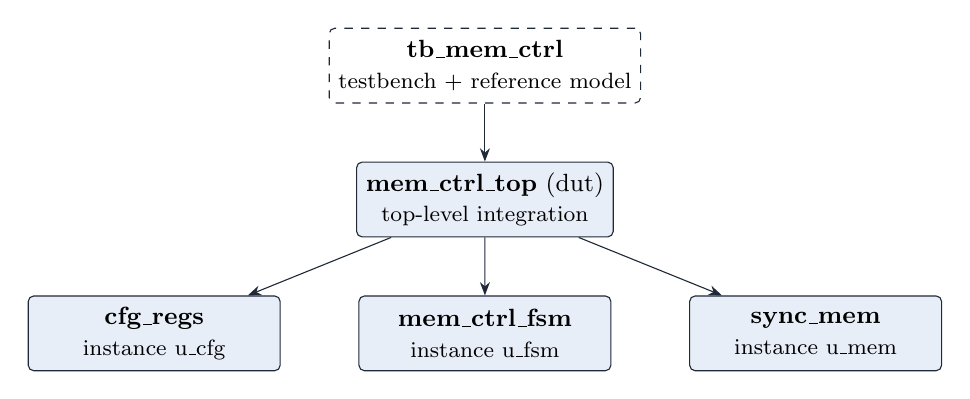
\begin{tikzpicture}[font=\small, >=Stealth,
  m/.style={draw=ink, fill=box, rounded corners=2pt, align=center, minimum width=3.2cm, minimum height=0.95cm},
  level distance=1.7cm, sibling distance=4.2cm, edge from parent/.style={draw=ink,->}]
\node[m, fill=white, dashed] {\textbf{tb\_mem\_ctrl}\\\footnotesize testbench + reference model}
  child {node[m] {\textbf{mem\_ctrl\_top} (dut)\\\footnotesize top-level integration}
    child {node[m] {\textbf{cfg\_regs}\\\footnotesize instance u\_cfg}}
    child {node[m] {\textbf{mem\_ctrl\_fsm}\\\footnotesize instance u\_fsm}}
    child {node[m] {\textbf{sync\_mem}\\\footnotesize instance u\_mem}}
  };
\end{tikzpicture}
\caption{Module hierarchy}
\label{fig:hier}
\end{figure}

\begin{table}[H]
\centering
\caption{Source files and responsibilities}
\label{tab:files}
\small
\begin{tabularx}{\textwidth}{@{}l l X@{}}
\toprule
\textbf{File} & \textbf{Module} & \textbf{Responsibility} \\
\midrule
\sig{rtl/mem\_ctrl\_top.v} & \sig{mem\_ctrl\_top} & Structural top; wires the three sub-blocks \\
\sig{rtl/mem\_ctrl\_fsm.v} & \sig{mem\_ctrl\_fsm} & State machine, request latch, validation, wait counter, error events \\
\sig{rtl/cfg\_regs.v} & \sig{cfg\_regs} & CTRL, WAIT, LIMIT, STATUS registers and read-back mux \\
\sig{rtl/sync\_mem.v} & \sig{sync\_mem} & 16 $\times$ 8 register-array memory, synchronous write, registered read \\
\sig{tb/tb\_mem\_ctrl.v} & \sig{tb\_mem\_ctrl} & Self-checking testbench with reference model \\
\bottomrule
\end{tabularx}
\end{table}

%======================== 5 FSM ========================
\section{FSM Diagram}
\begin{figure}[H]
\centering
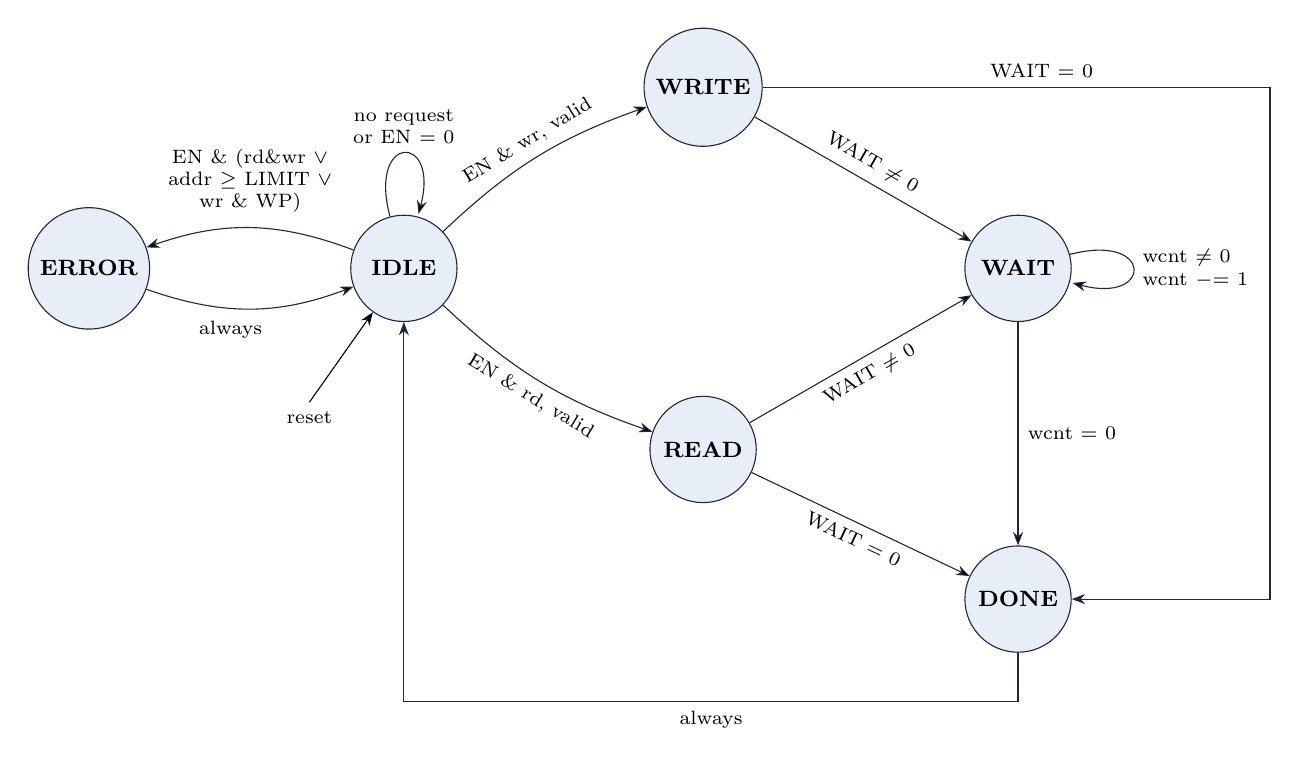
\begin{tikzpicture}[>=Stealth, font=\scriptsize, node distance=2cm,
  every state/.style={draw=ink, fill=box, minimum size=1.35cm, font=\footnotesize\bfseries}]
\node[state] (idle)  at (0,0)    {IDLE};
\node[state] (err)   at (-4.0,0) {ERROR};
\node[state] (wr)    at (3.8,2.3)  {WRITE};
\node[state] (rd)    at (3.8,-2.3) {READ};
\node[state] (wait)  at (7.8,0)  {WAIT};
\node[state] (done)  at (7.8,-4.2) {DONE};
\draw[->] (-1.2,-1.7) node[below,font=\scriptsize]{reset} -- (idle);
\path[->,draw=ink]
 (idle) edge[loop above] node[above,align=center]{no request\\or EN = 0} ()
 (idle) edge[bend left=12] node[above,sloped,align=center]{EN \& wr, valid} (wr)
 (idle) edge[bend right=12] node[below,sloped]{EN \& rd, valid} (rd)
 (idle) edge[bend right=20] node[above=2pt,align=center]{EN \& (rd\&wr $\vee$\\addr $\ge$ LIMIT $\vee$\\wr \& WP)} (err)
 (err)  edge[bend right=20] node[below=1pt,pos=0.4]{always} (idle)
 (wr)   edge node[above,sloped]{WAIT $\ne$ 0} (wait)
 (rd)   edge node[below,sloped]{WAIT $\ne$ 0} (wait)
 (rd)   edge node[below,sloped]{WAIT = 0} (done)
 (wait) edge[loop right] node[right,align=left]{wcnt $\ne$ 0\\wcnt $-$= 1} ()
 (wait) edge node[right]{wcnt = 0} (done);
\draw[->,draw=ink] (wr.east) -- (11.0,2.3) node[pos=0.55,above]{WAIT = 0} |- (done.east);
\draw[->,draw=ink] (done.south) -- (7.8,-5.5) -| node[pos=0.25,below]{always} (idle.south);
\end{tikzpicture}
\caption{Controller state transition diagram (Moore machine)}
\label{fig:fsm}
\end{figure}

\begin{table}[H]
\centering
\caption{State encoding and Moore outputs}
\label{tab:states}
\small
\begin{tabularx}{\textwidth}{@{}l c c c c c c X@{}}
\toprule
\textbf{State} & \textbf{Code} & \sig{busy} & \sig{ready} & \sig{error} & \sig{mem\_we} & \sig{mem\_re} & \textbf{Action} \\
\midrule
IDLE  & 000 & 0 & 0 & 0 & 0 & 0 & Wait for request, latch and validate it \\
READ  & 001 & 1 & 0 & 0 & 0 & 1 & Memory read strobe; data registered at end of cycle \\
WRITE & 010 & 1 & 0 & 0 & 1 & 0 & Memory write strobe; array updated at end of cycle \\
WAIT  & 011 & 1 & 0 & 0 & 0 & 0 & Count down the programmed wait states \\
DONE  & 100 & 1 & 1 & 0 & 0 & 0 & Signal completion; \sig{read\_data} valid \\
ERROR & 101 & 1 & 1 & 1 & 0 & 0 & Signal rejection; memory not accessed \\
\bottomrule
\end{tabularx}
\end{table}
Binary encoding was kept deliberately: with six states it needs three flip-flops, and Yosys reported that re-encoding would bring no benefit for this output decode.

%======================== 6 DATAPATH ========================
\section{Datapath Diagram}
\begin{figure}[H]
\centering
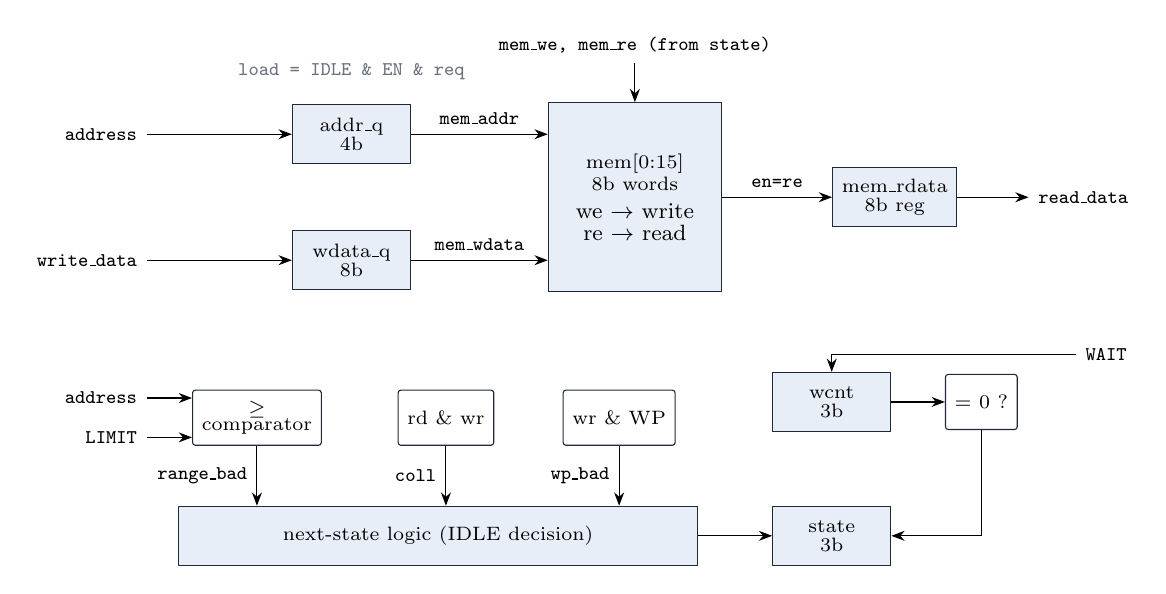
\begin{tikzpicture}[>=Stealth, font=\scriptsize,
  r/.style={draw=ink, fill=box, minimum width=1.5cm, minimum height=0.75cm, align=center},
  c/.style={draw=ink, fill=white, align=center, minimum height=0.7cm, rounded corners=1pt},
  t/.style={font=\scriptsize\ttfamily}]
% request latch
\node[r] (aq) at (0,1.6) {addr\_q\\[-1pt]4b};
\node[r] (wq) at (0,0)   {wdata\_q\\[-1pt]8b};
\draw[->] (-2.6,1.6) node[left,t]{address} -- (aq);
\draw[->] (-2.6,0) node[left,t]{write\_data} -- (wq);
\node[t, color=mut] at (0,2.4) {load = IDLE \& EN \& req};
% memory
\node[r, minimum width=2.2cm, minimum height=2.4cm] (ram) at (3.6,0.8) {mem[0:15]\\8b words\\[2pt]\footnotesize we $\to$ write\\\footnotesize re $\to$ read};
\draw[->] (aq) -- node[above,t]{mem\_addr} (ram.west |- aq);
\draw[->] (wq) -- node[above,t]{mem\_wdata} (ram.west |- wq);
\node[r] (rq) at (6.9,0.8) {mem\_rdata\\[-1pt]8b reg};
\draw[->] (ram) -- node[above,t]{en=re} (rq);
\draw[->] (rq) -- (8.6,0.8) node[right,t]{read\_data};
\draw[<-] (ram.north) -- ++(0,0.5) node[above,t]{mem\_we, mem\_re (from state)};
% validation
\node[c] (cmp) at (-1.2,-2.0) {$\geq$\\[-2pt]comparator};
\node[c] (and1) at (1.2,-2.0) {rd \& wr};
\node[c] (and2) at (3.4,-2.0) {wr \& WP};
\draw[->] (-2.6,-1.75) node[left,t]{address} -- (cmp.west |- 0,-1.75);
\draw[->] (-2.6,-2.25) node[left,t]{LIMIT} -- (cmp.west |- 0,-2.25);
\node[r, minimum width=6.6cm] (nsl) at (1.1,-3.5) {next-state logic (IDLE decision)};
\draw[->] (cmp) -- node[left,t]{range\_bad} (cmp |- nsl.north);
\draw[->] (and1) -- node[left,t]{coll} (and1 |- nsl.north);
\draw[->] (and2) -- node[left,t]{wp\_bad} (and2 |- nsl.north);
\node[r] (st) at (6.1,-3.5) {state\\[-1pt]3b};
\draw[->] (nsl) -- (st);
% wait counter
\node[r] (wc) at (6.1,-1.8) {wcnt\\[-1pt]3b};
\node[c] (z) at (8.0,-1.8) {= 0 ?};
\draw[->] (wc) -- (z);
\draw[->] (z) |- (st.east);
\draw[->] (9.2,-1.2) node[right,t]{WAIT} -| (wc.north);
\end{tikzpicture}
\caption{Datapath: request latch, memory array, read register, validation logic and wait counter}
\label{fig:dp}
\end{figure}
The longest combinational path in the design runs from \sig{address} and the LIMIT register through the $\geq$ comparator and the IDLE next-state decision into the state register (Section~\ref{sec:timing}). All memory-side signals leave registers directly (\sig{addr\_q}, \sig{wdata\_q}, state decode), so the memory write and read paths are short.

%======================== 7 RTL ========================
\section{RTL Source Code}
All modules are written in synthesizable Verilog-2005. Sequential logic uses non-blocking assignments in clocked \sig{always} blocks; combinational logic uses \sig{always @(*)} with a default assignment at the top so that no latches are inferred. The \sig{initial} block in \sig{sync\_mem} only sets the power-up contents of the array, which Vivado honours as an FPGA initial value.

\subsection{mem\_ctrl\_top.v}
\begin{lstlisting}
//============================================================================
// Module      : mem_ctrl_top
// Project     : MOSART Project 8 - Programmable Memory Controller
// Author      : Shaun Praneeth Raj
// Description : Top level. Connects the configuration register bank, the
//               controller FSM and the 16 x 8 synchronous register-array
//               memory. All logic is in a single clock domain (clk) with a
//               synchronous active-high reset.
//============================================================================
`timescale 1ns / 1ps
module mem_ctrl_top #(
    parameter DATA_W = 8,
    parameter ADDR_W = 4
)(
    input  wire              clk,
    input  wire              reset,
    // host request interface
    input  wire              read_enable,
    input  wire              write_enable,
    input  wire [ADDR_W-1:0] address,
    input  wire [DATA_W-1:0] write_data,
    output wire [DATA_W-1:0] read_data,
    output wire              ready,
    output wire              busy,
    output wire              error,
    // configuration interface
    input  wire              cfg_we,
    input  wire [1:0]        cfg_addr,
    input  wire [7:0]        cfg_wdata,
    output wire [7:0]        cfg_rdata
);
    wire              en, wp;
    wire [2:0]        wait_states;
    wire [ADDR_W:0]   addr_limit;
    wire              mem_we, mem_re;
    wire [ADDR_W-1:0] mem_addr;
    wire [DATA_W-1:0] mem_wdata;
    wire              ev_coll, ev_range, ev_wpv, ev_ovr;

    cfg_regs #(.ADDR_W(ADDR_W)) u_cfg (
        .clk(clk), .reset(reset),
        .cfg_we(cfg_we), .cfg_addr(cfg_addr),
        .cfg_wdata(cfg_wdata), .cfg_rdata(cfg_rdata),
        .en(en), .wp(wp), .wait_states(wait_states), .addr_limit(addr_limit),
        .ev_coll(ev_coll), .ev_range(ev_range), .ev_wpv(ev_wpv),
        .ev_ovr(ev_ovr), .busy(busy)
    );

    mem_ctrl_fsm #(.DATA_W(DATA_W), .ADDR_W(ADDR_W)) u_fsm (
        .clk(clk), .reset(reset),
        .read_enable(read_enable), .write_enable(write_enable),
        .address(address), .write_data(write_data),
        .ready(ready), .busy(busy), .error(error),
        .en(en), .wp(wp), .wait_states(wait_states), .addr_limit(addr_limit),
        .mem_we(mem_we), .mem_re(mem_re),
        .mem_addr(mem_addr), .mem_wdata(mem_wdata),
        .ev_coll(ev_coll), .ev_range(ev_range), .ev_wpv(ev_wpv), .ev_ovr(ev_ovr)
    );

    sync_mem #(.DATA_W(DATA_W), .ADDR_W(ADDR_W)) u_mem (
        .clk(clk),
        .mem_we(mem_we), .mem_re(mem_re),
        .mem_addr(mem_addr), .mem_wdata(mem_wdata),
        .mem_rdata(read_data)
    );
endmodule
\end{lstlisting}
\subsection{mem\_ctrl\_fsm.v}
\begin{lstlisting}
//============================================================================
// Module      : mem_ctrl_fsm
// Project     : MOSART Project 8 - Programmable Memory Controller
// Author      : Shaun Praneeth Raj
// Description : Control path. Accepts one request at a time from the host,
//               validates it, drives the memory strobes, inserts the
//               programmed number of wait states and signals completion.
//
//   States : IDLE -> READ  -> [WAIT] -> DONE -> IDLE
//            IDLE -> WRITE -> [WAIT] -> DONE -> IDLE
//            IDLE -> ERROR -> IDLE              (rejected request)
//
//   busy  = 1 in every state except IDLE
//   ready = 1 for one cycle in DONE or ERROR (transaction finished)
//   error = 1 for one cycle in ERROR (request rejected, memory untouched)
//============================================================================
`timescale 1ns / 1ps
module mem_ctrl_fsm #(
    parameter DATA_W = 8,
    parameter ADDR_W = 4
)(
    input  wire              clk,
    input  wire              reset,
    // host request interface
    input  wire              read_enable,
    input  wire              write_enable,
    input  wire [ADDR_W-1:0] address,
    input  wire [DATA_W-1:0] write_data,
    output wire              ready,
    output wire              busy,
    output wire              error,
    // programmed configuration
    input  wire              en,
    input  wire              wp,
    input  wire [2:0]        wait_states,
    input  wire [ADDR_W:0]   addr_limit,
    // memory control
    output wire              mem_we,
    output wire              mem_re,
    output wire [ADDR_W-1:0] mem_addr,
    output wire [DATA_W-1:0] mem_wdata,
    // error events to the status register
    output reg               ev_coll,
    output reg               ev_range,
    output reg               ev_wpv,
    output reg               ev_ovr
);
    localparam [2:0] S_IDLE  = 3'd0,
                     S_READ  = 3'd1,
                     S_WRITE = 3'd2,
                     S_WAIT  = 3'd3,
                     S_DONE  = 3'd4,
                     S_ERROR = 3'd5;

    reg [2:0]        state, next_state;
    reg [ADDR_W-1:0] addr_q;
    reg [DATA_W-1:0] wdata_q;
    reg [2:0]        wcnt;

    wire req      = read_enable | write_enable;
    wire coll     = read_enable & write_enable;
    wire range_bad = ({1'b0, address} >= addr_limit);
    wire wp_bad   = write_enable & wp;

    // ---------------- next-state logic ----------------
    always @(*) begin
        next_state = state;
        case (state)
            S_IDLE:
                if (en && req) begin
                    if (coll || range_bad || wp_bad) next_state = S_ERROR;
                    else if (write_enable)           next_state = S_WRITE;
                    else                             next_state = S_READ;
                end
            S_READ,
            S_WRITE: next_state = (wait_states != 3'd0) ? S_WAIT : S_DONE;
            S_WAIT : next_state = (wcnt == 3'd0) ? S_DONE : S_WAIT;
            S_DONE : next_state = S_IDLE;
            S_ERROR: next_state = S_IDLE;
            default: next_state = S_IDLE;
        endcase
    end

    // ---------------- state, request latch, wait counter ----------------
    always @(posedge clk) begin
        if (reset) begin
            state   <= S_IDLE;
            addr_q  <= {ADDR_W{1'b0}};
            wdata_q <= {DATA_W{1'b0}};
            wcnt    <= 3'd0;
        end else begin
            state <= next_state;
            if (state == S_IDLE && en && req) begin
                addr_q  <= address;
                wdata_q <= write_data;
            end
            if ((state == S_READ || state == S_WRITE) && wait_states != 3'd0)
                wcnt <= wait_states - 3'd1;
            else if (state == S_WAIT && wcnt != 3'd0)
                wcnt <= wcnt - 3'd1;
        end
    end

    // ---------------- error event pulses (registered) ----------------
    always @(posedge clk) begin
        if (reset) begin
            ev_coll <= 1'b0; ev_range <= 1'b0; ev_wpv <= 1'b0; ev_ovr <= 1'b0;
        end else begin
            ev_coll  <= (state == S_IDLE) && en && coll;
            ev_range <= (state == S_IDLE) && en && req && !coll && range_bad;
            ev_wpv   <= (state == S_IDLE) && en && !coll && !range_bad && wp_bad;
            ev_ovr   <= (state != S_IDLE) && req;
        end
    end

    // ---------------- Moore outputs ----------------
    assign busy      = (state != S_IDLE);
    assign ready     = (state == S_DONE) || (state == S_ERROR);
    assign error     = (state == S_ERROR);
    assign mem_we    = (state == S_WRITE);
    assign mem_re    = (state == S_READ);
    assign mem_addr  = addr_q;
    assign mem_wdata = wdata_q;
endmodule
\end{lstlisting}
\subsection{cfg\_regs.v}
\begin{lstlisting}
//============================================================================
// Module      : cfg_regs
// Project     : MOSART Project 8 - Programmable Memory Controller
// Author      : Shaun Praneeth Raj
// Description : Configuration and status register bank. Programs the
//               controller behaviour at run time.
//
//   Addr  Name    Bits   Access  Reset  Meaning
//   0x0   CTRL    [0]    RW      1      EN  : controller enable
//                 [1]    RW      0      WP  : write protect (writes rejected)
//   0x1   WAIT    [2:0]  RW      0      number of wait states per access
//   0x2   LIMIT   [4:0]  RW      16     number of valid words (addr < LIMIT)
//   0x3   STATUS  [0]    W1C     0      COLL : simultaneous read+write request
//                 [1]    W1C     0      RANGE: address >= LIMIT
//                 [2]    W1C     0      WPV  : write attempted while WP = 1
//                 [3]    W1C     0      OVR  : request dropped while busy
//                 [4]    RO      -      BUSY : controller busy (live)
//                 [7:5]  RO      0      reserved
//============================================================================
`timescale 1ns / 1ps
module cfg_regs #(
    parameter ADDR_W = 4
)(
    input  wire          clk,
    input  wire          reset,       // synchronous, active high
    // configuration port
    input  wire          cfg_we,
    input  wire [1:0]    cfg_addr,
    input  wire [7:0]    cfg_wdata,
    output reg  [7:0]    cfg_rdata,
    // decoded controls to the FSM
    output reg           en,
    output reg           wp,
    output reg  [2:0]    wait_states,
    output reg  [ADDR_W:0] addr_limit,
    // error events from the FSM (one-cycle pulses)
    input  wire          ev_coll,
    input  wire          ev_range,
    input  wire          ev_wpv,
    input  wire          ev_ovr,
    input  wire          busy
);
    localparam A_CTRL = 2'd0, A_WAIT = 2'd1, A_LIMIT = 2'd2, A_STAT = 2'd3;

    reg [3:0] sticky;   // {OVR, WPV, RANGE, COLL}

    wire [3:0] clr = (cfg_we && cfg_addr == A_STAT) ? cfg_wdata[3:0] : 4'b0;
    wire [3:0] set = {ev_ovr, ev_wpv, ev_range, ev_coll};

    always @(posedge clk) begin
        if (reset) begin
            en          <= 1'b1;
            wp          <= 1'b0;
            wait_states <= 3'd0;
            addr_limit  <= (1 << ADDR_W);
            sticky      <= 4'b0;
        end else begin
            if (cfg_we) begin
                case (cfg_addr)
                    A_CTRL : begin en <= cfg_wdata[0]; wp <= cfg_wdata[1]; end
                    A_WAIT : wait_states <= cfg_wdata[2:0];
                    A_LIMIT: addr_limit  <= (cfg_wdata[ADDR_W:0] > (1 << ADDR_W))
                                            ? (1 << ADDR_W) : cfg_wdata[ADDR_W:0];
                    default: ;
                endcase
            end
            // a new event in the same cycle wins over the clear
            sticky <= (sticky & ~clr) | set;
        end
    end

    // combinational read-back
    always @(*) begin
        case (cfg_addr)
            A_CTRL : cfg_rdata = {6'b0, wp, en};
            A_WAIT : cfg_rdata = {5'b0, wait_states};
            A_LIMIT: cfg_rdata = {{(7-ADDR_W){1'b0}}, addr_limit};
            default: cfg_rdata = {3'b0, busy, sticky};
        endcase
    end
endmodule
\end{lstlisting}
\subsection{sync\_mem.v}
\begin{lstlisting}
//============================================================================
// Module      : sync_mem
// Project     : MOSART Project 8 - Programmable Memory Controller
// Author      : Shaun Praneeth Raj
// Description : Single-port synchronous on-chip memory built from a register
//               array. Write is synchronous; read data is registered, so the
//               word addressed while mem_re is high appears on dout one clock
//               later and is held until the next read.
//============================================================================
`timescale 1ns / 1ps
module sync_mem #(
    parameter DATA_W = 8,
    parameter ADDR_W = 4
)(
    input  wire              clk,
    input  wire              mem_we,
    input  wire              mem_re,
    input  wire [ADDR_W-1:0] mem_addr,
    input  wire [DATA_W-1:0] mem_wdata,
    output reg  [DATA_W-1:0] mem_rdata
);
    localparam DEPTH = (1 << ADDR_W);

    reg [DATA_W-1:0] mem [0:DEPTH-1];

    integer i;
    initial begin
        for (i = 0; i < DEPTH; i = i + 1)
            mem[i] = {DATA_W{1'b0}};
        mem_rdata = {DATA_W{1'b0}};
    end

    always @(posedge clk) begin
        if (mem_we)
            mem[mem_addr] <= mem_wdata;
        if (mem_re)
            mem_rdata <= mem[mem_addr];
    end
endmodule
\end{lstlisting}

%======================== 8 TESTBENCH ========================
\section{Testbench}
The testbench \sig{tb\_mem\_ctrl} instantiates \sig{mem\_ctrl\_top} with a 100 MHz clock. Stimulus is applied on the falling edge and outputs are sampled on the falling edge after the rising edge that produced them, which removes any race between testbench and design. A reference array \sig{model[]} is updated only by accepted writes; every read is compared against it. Reusable tasks (\sig{cfg\_write}, \sig{cfg\_expect}, \sig{do\_access}, \sig{mem\_write}, \sig{mem\_read}) keep the test sequences short, and \sig{do\_access} also measures the latency of each transaction and checks that \sig{busy} stays high until \sig{ready}.

\begin{table}[H]
\centering
\caption{Verification plan}
\label{tab:plan}
\small
\begin{tabularx}{\textwidth}{@{}l X X@{}}
\toprule
\textbf{Test} & \textbf{Scenario} & \textbf{Checks} \\
\midrule
T1 & Reset values & CTRL = 0x01, WAIT = 0, LIMIT = 16, STATUS = 0, busy and ready low \\
T2 & Write all 16 words, read all back, WAIT = 0 & Data integrity at every address; latency = 2 cycles \\
T3 & WAIT programmed to 1 through 7 & Latency = 2 + WAIT for both reads and writes; busy held throughout \\
T4 & \sig{read\_enable} and \sig{write\_enable} together & error pulse, STATUS.COLL set, memory unchanged, W1C clear \\
T5 & LIMIT = 8, access 0xA and 0xC, then 0x7 & RANGE error for out-of-window, normal access at 0x7, oversize LIMIT saturates to 16 \\
T6 & WP = 1 and a write & WPV error, memory unchanged, reads still allowed \\
T7 & Second request while busy (WAIT = 4) & Request dropped, STATUS.OVR set, first write completes \\
T8 & EN = 0 with request held for four cycles & busy and ready stay low, memory unchanged \\
T9 & Reset during a read with WAIT = 5 & FSM returns to IDLE, configuration to defaults, memory contents preserved \\
T10 & 500 random reads and writes, WAIT re-randomised every 50 accesses, then full read-back & Every read matches the reference model \\
\bottomrule
\end{tabularx}
\end{table}

\begin{lstlisting}
//============================================================================
// Testbench   : tb_mem_ctrl
// Project     : MOSART Project 8 - Programmable Memory Controller
// Author      : Shaun Praneeth Raj
// Description : Self-checking testbench. A behavioural reference model
//               (model[]) mirrors every accepted write; every read and every
//               status/config read-back is compared against it. Stimulus is
//               driven on the falling edge, outputs are sampled on the
//               rising edge. Ends with a PASS/FAIL summary.
//============================================================================
`timescale 1ns/1ps
module tb_mem_ctrl;
    localparam DATA_W = 8, ADDR_W = 4, DEPTH = 16;
    localparam CLK_P  = 10;                         // 100 MHz

    reg               clk = 0, reset = 1;
    reg               read_enable = 0, write_enable = 0;
    reg  [ADDR_W-1:0] address = 0;
    reg  [DATA_W-1:0] write_data = 0;
    wire [DATA_W-1:0] read_data;
    wire              ready, busy, error;
    reg               cfg_we = 0;
    reg  [1:0]        cfg_addr = 0;
    reg  [7:0]        cfg_wdata = 0;
    wire [7:0]        cfg_rdata;

    mem_ctrl_top #(.DATA_W(DATA_W), .ADDR_W(ADDR_W)) dut (
        .clk(clk), .reset(reset),
        .read_enable(read_enable), .write_enable(write_enable),
        .address(address), .write_data(write_data), .read_data(read_data),
        .ready(ready), .busy(busy), .error(error),
        .cfg_we(cfg_we), .cfg_addr(cfg_addr),
        .cfg_wdata(cfg_wdata), .cfg_rdata(cfg_rdata)
    );

    always #(CLK_P/2) clk = ~clk;

    // ---------------- reference model & bookkeeping ----------------
    reg [DATA_W-1:0] model [0:DEPTH-1];
    integer errors = 0, checks = 0, test_errors_start = 0;
    integer lat, k, n, a, d, op, ws;
    integer n_rd = 0, n_wr = 0, n_rej = 0;
    reg [7:0] cur_wait = 0;
    reg [4:0] cur_limit = 16;
    reg       cur_wp = 0;
    reg       got_err;

    task check(input [639:0] what, input [31:0] got, input [31:0] exp);
        begin
            checks = checks + 1;
            if (got !== exp) begin
                errors = errors + 1;
                $display("  ** FAIL %0s : got 0x%0h expected 0x%0h @ %0t",
                         what, got, exp, $time);
            end
        end
    endtask

    task begin_test(input [639:0] name);
        begin
            test_errors_start = errors;
            $display("[%0t] TEST: %0s", $time, name);
        end
    endtask

    task end_test(input [639:0] name);
        begin
            if (errors == test_errors_start) $display("    -> PASS  %0s", name);
            else                             $display("    -> FAIL  %0s", name);
        end
    endtask

    // ---------------- config bus ----------------
    task cfg_write(input [1:0] ad, input [7:0] dat);
        begin
            @(negedge clk); cfg_we = 1; cfg_addr = ad; cfg_wdata = dat;
            @(negedge clk); cfg_we = 0;
        end
    endtask

    task cfg_expect(input [1:0] ad, input [7:0] exp);
        begin
            @(negedge clk); cfg_addr = ad; #1;
            check("cfg readback", cfg_rdata, exp);
        end
    endtask

    // ---------------- host transactions ----------------
    // Issues one request, waits for ready, returns latency (cycles from the
    // edge that samples the request to the edge that samples ready) and
    // whether the controller flagged an error.
    task do_access(input rd, input wr, input [ADDR_W-1:0] ad,
                   input [DATA_W-1:0] dat, output integer cycles,
                   output reg err);
        begin
            @(negedge clk);
            read_enable = rd; write_enable = wr; address = ad; write_data = dat;
            @(negedge clk);
            read_enable = 0; write_enable = 0;
            cycles = 1;
            while (!ready) begin
                check("busy during access", busy, 1);
                @(negedge clk); cycles = cycles + 1;
            end
            err = error;
        end
    endtask

    task mem_write(input [ADDR_W-1:0] ad, input [DATA_W-1:0] dat,
                   input exp_err);
        begin
            do_access(0, 1, ad, dat, lat, got_err);
            check("write error flag", got_err, exp_err);
            if (!got_err) begin model[ad] = dat; n_wr = n_wr + 1; end
            else n_rej = n_rej + 1;
        end
    endtask

    task mem_read(input [ADDR_W-1:0] ad, input exp_err);
        begin
            do_access(1, 0, ad, 8'h00, lat, got_err);
            check("read error flag", got_err, exp_err);
            if (!got_err) begin
                check("read data", read_data, model[ad]);
                n_rd = n_rd + 1;
            end else n_rej = n_rej + 1;
        end
    endtask

    // ---------------- stimulus ----------------
    initial begin
        $dumpfile("mem_ctrl.vcd");
        $dumpvars(0, tb_mem_ctrl);
        for (k = 0; k < DEPTH; k = k + 1) model[k] = 0;

        repeat (3) @(negedge clk);
        reset = 0;

        //--------------------------------------------------------------
        begin_test("T1 reset values of configuration registers");
        cfg_expect(2'd0, 8'h01);   // EN=1, WP=0
        cfg_expect(2'd1, 8'h00);   // WAIT=0
        cfg_expect(2'd2, 8'h10);   // LIMIT=16
        cfg_expect(2'd3, 8'h00);   // STATUS clear, not busy
        check("busy after reset", busy, 0);
        check("ready after reset", ready, 0);
        end_test("T1");

        //--------------------------------------------------------------
        begin_test("T2 write all 16 words, read back, zero wait states");
        for (k = 0; k < DEPTH; k = k + 1) begin
            mem_write(k, 8'hA0 ^ (k * 8'h11), 0);
            check("write latency WAIT=0", lat, 2);
        end
        for (k = 0; k < DEPTH; k = k + 1) begin
            mem_read(k, 0);
            check("read latency WAIT=0", lat, 2);
        end
        end_test("T2");

        //--------------------------------------------------------------
        begin_test("T3 programmable wait states 1..7");
        for (ws = 1; ws < 8; ws = ws + 1) begin
            cfg_write(2'd1, ws);
            mem_write(ws, 8'h30 + ws, 0);
            check("write latency", lat, 2 + ws);
            mem_read(ws, 0);
            check("read latency", lat, 2 + ws);
        end
        cfg_write(2'd1, 8'd3);
        mem_write(4'hF, 8'h5A, 0);
        mem_read (4'hF, 0);
        check("read latency WAIT=3", lat, 5);
        cfg_write(2'd1, 8'd0);
        end_test("T3");

        //--------------------------------------------------------------
        begin_test("T4 simultaneous read + write request is rejected");
        do_access(1, 1, 4'h2, 8'hEE, lat, got_err);
        check("collision error", got_err, 1);
        n_rej = n_rej + 1;
        cfg_expect(2'd3, 8'h01);   // COLL set
        mem_read(4'h2, 0);         // memory must be unchanged
        cfg_write(2'd3, 8'h01);    // W1C
        cfg_expect(2'd3, 8'h00);
        end_test("T4");

        //--------------------------------------------------------------
        begin_test("T5 address limit (LIMIT = 8)");
        cfg_write(2'd2, 8'd8);
        cfg_expect(2'd2, 8'd8);
        mem_write(4'd10, 8'h99, 1);    // out of range -> error
        mem_read (4'd12, 1);
        cfg_expect(2'd3, 8'h02);       // RANGE set
        mem_write(4'd7, 8'h77, 0);     // last valid word
        mem_read (4'd7, 0);
        cfg_write(2'd2, 8'd31);        // oversize value saturates to 16
        cfg_expect(2'd2, 8'd16);
        mem_read (4'd10, 0);           // old contents intact
        cfg_write(2'd3, 8'h0F);
        end_test("T5");

        //--------------------------------------------------------------
        begin_test("T6 write protect");
        cfg_write(2'd0, 8'h03);        // EN=1, WP=1
        mem_write(4'd3, 8'hFF, 1);
        cfg_expect(2'd3, 8'h04);       // WPV set
        mem_read (4'd3, 0);            // reads still allowed, data unchanged
        cfg_write(2'd0, 8'h01);
        cfg_write(2'd3, 8'h0F);
        mem_write(4'd3, 8'h3C, 0);
        mem_read (4'd3, 0);
        end_test("T6");

        //--------------------------------------------------------------
        begin_test("T7 request while busy is dropped and flagged");
        cfg_write(2'd1, 8'd4);
        @(negedge clk);
        write_enable = 1; address = 4'd5; write_data = 8'h55;
        @(negedge clk);
        write_enable = 1; address = 4'd6; write_data = 8'h66;  // arrives while busy
        @(negedge clk);
        write_enable = 0;
        while (!ready) @(negedge clk);
        model[5] = 8'h55; n_wr = n_wr + 1;
        cfg_expect(2'd3, 8'h08);       // OVR set
        mem_read(4'd6, 0);             // location 6 must NOT be 0x66
        mem_read(4'd5, 0);
        cfg_write(2'd3, 8'h0F);
        cfg_write(2'd1, 8'd0);
        end_test("T7");

        //--------------------------------------------------------------
        begin_test("T8 controller disabled (EN = 0) ignores requests");
        cfg_write(2'd0, 8'h00);
        @(negedge clk);
        write_enable = 1; address = 4'd1; write_data = 8'hBD;
        repeat (4) begin
            @(negedge clk);
            check("busy while disabled", busy, 0);
            check("ready while disabled", ready, 0);
        end
        write_enable = 0;
        cfg_write(2'd0, 8'h01);
        mem_read(4'd1, 0);             // not overwritten
        end_test("T8");

        //--------------------------------------------------------------
        begin_test("T9 reset during a transaction");
        cfg_write(2'd1, 8'd5);
        @(negedge clk);
        read_enable = 1; address = 4'd9;
        @(negedge clk); read_enable = 0;
        @(negedge clk); @(negedge clk);
        check("busy mid-transaction", busy, 1);
        reset = 1; @(negedge clk); reset = 0;
        check("busy after reset", busy, 0);
        cfg_expect(2'd1, 8'd0);        // config back to default
        mem_read(4'd9, 0);             // memory array keeps its contents
        end_test("T9");

        //--------------------------------------------------------------
        begin_test("T10 constrained-random regression (500 accesses)");
        n = 0;
        for (k = 0; k < 500; k = k + 1) begin
            if (k % 50 == 0) begin
                cfg_write(2'd1, $urandom % 8);
            end
            a  = $urandom % DEPTH;
            d  = $urandom % 256;
            op = $urandom % 2;
            if (op) mem_write(a, d, 0);
            else    mem_read (a, 0);
        end
        for (k = 0; k < DEPTH; k = k + 1) mem_read(k, 0);
        end_test("T10");

        //--------------------------------------------------------------
        repeat (3) @(negedge clk);
        $display("============================================================");
        $display(" SUMMARY: %0d checks, %0d errors | %0d writes, %0d reads, %0d rejected",
                 checks, errors, n_wr, n_rd, n_rej);
        if (errors == 0) $display(" RESULT : ALL TESTS PASSED");
        else             $display(" RESULT : FAILURES DETECTED");
        $display("============================================================");
        $finish;
    end

    // watchdog
    initial begin
        #2_000_000;
        $display("TIMEOUT"); $finish;
    end
endmodule
\end{lstlisting}

%======================== 9 SIMULATION ========================
\section{Simulation Results}

\subsection{Simulation Log}
The testbench was compiled and run with Icarus Verilog 12.0 (\sig{iverilog -g2005}). The same sources can be run in the Vivado simulator with \sig{vivado/run\_sim.tcl}. The console output is reproduced below.

\begin{lstlisting}[language={},basicstyle=\ttfamily\scriptsize,numbers=none]
[30 ns]   TEST: T1 reset values of configuration registers        -> PASS
[71 ns]   TEST: T2 write all 16 words, read back, zero wait states -> PASS
[1030 ns] TEST: T3 programmable wait states 1..7                   -> PASS
[2310 ns] TEST: T4 simultaneous read + write request is rejected   -> PASS
[2401 ns] TEST: T5 address limit (LIMIT = 8)                       -> PASS
[2620 ns] TEST: T6 write protect                                   -> PASS
[2800 ns] TEST: T7 request while busy is dropped and flagged       -> PASS
[3080 ns] TEST: T8 controller disabled (EN = 0) ignores requests   -> PASS
[3200 ns] TEST: T9 reset during a transaction                      -> PASS
[3310 ns] TEST: T10 constrained-random regression (500 accesses)   -> PASS
============================================================
 SUMMARY: 3356 checks, 0 errors | 281 writes, 295 reads, 4 rejected
 RESULT : ALL TESTS PASSED
============================================================
$finish called at 36680 ns
\end{lstlisting}

To confirm that the checker is capable of detecting faults, two deliberate bugs were injected into a copy of the FSM. Removing the collision check made T4 fail (2 errors), and loading the wait counter with \sig{WAIT} instead of \sig{WAIT}~$-$~1 made T3 fail (15 latency errors). The original RTL passes every check.

\subsection{Simulation Waveforms}
All waveforms below are drawn in TikZ directly from the VCD dump of the passing run. Values on buses are hexadecimal unless stated otherwise; vertical grid lines mark rising clock edges.

\begin{figure}[H]
\centering
\resizebox{\textwidth}{!}{%
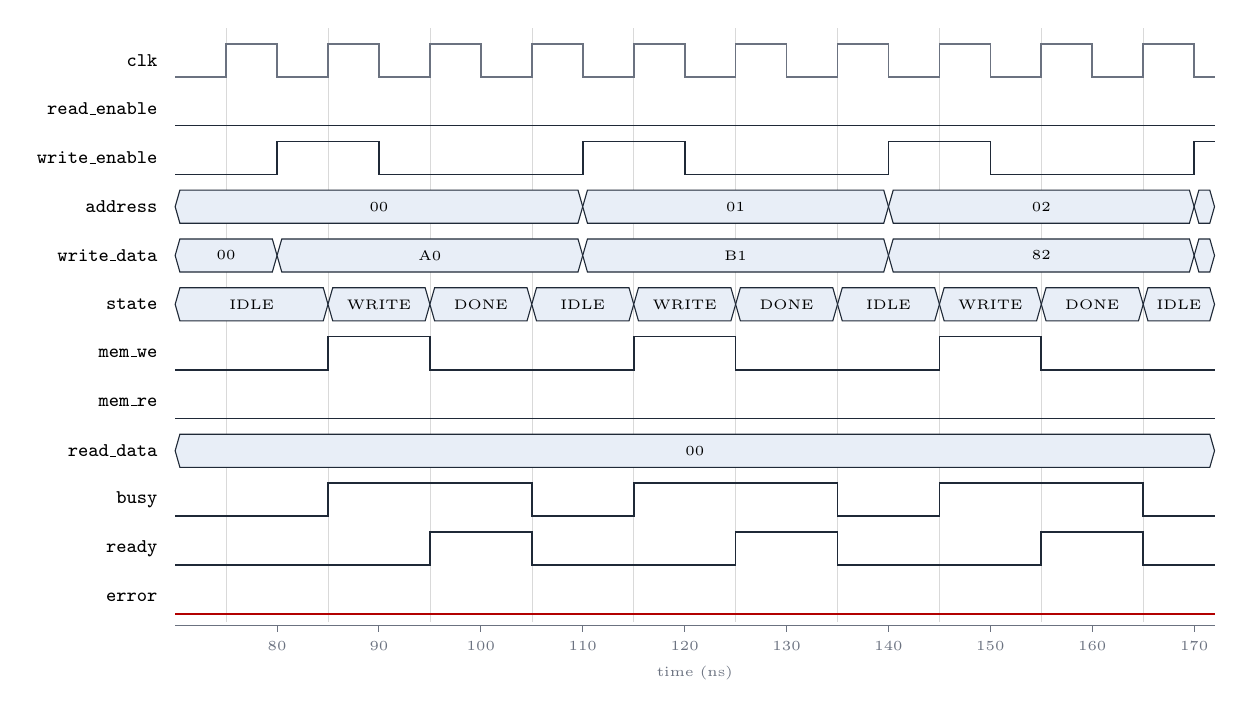
\begin{tikzpicture}[x=1cm,y=1cm,font=\scriptsize]
\draw[gray!30,very thin] (0.647,-0.1) -- (0.647,7.440);
\draw[gray!30,very thin] (1.941,-0.1) -- (1.941,7.440);
\draw[gray!30,very thin] (3.235,-0.1) -- (3.235,7.440);
\draw[gray!30,very thin] (4.529,-0.1) -- (4.529,7.440);
\draw[gray!30,very thin] (5.824,-0.1) -- (5.824,7.440);
\draw[gray!30,very thin] (7.118,-0.1) -- (7.118,7.440);
\draw[gray!30,very thin] (8.412,-0.1) -- (8.412,7.440);
\draw[gray!30,very thin] (9.706,-0.1) -- (9.706,7.440);
\draw[gray!30,very thin] (11.000,-0.1) -- (11.000,7.440);
\draw[gray!30,very thin] (12.294,-0.1) -- (12.294,7.440);
\node[anchor=east,font=\scriptsize\ttfamily] at (-0.1,7.030) {clk};
\draw[mut,line width=0.6pt] (0.000,6.820) -- (0.647,6.820) -- (0.647,7.240) -- (1.294,7.240) -- (1.294,6.820) -- (1.941,6.820) -- (1.941,7.240) -- (2.588,7.240) -- (2.588,6.820) -- (3.235,6.820) -- (3.235,7.240) -- (3.882,7.240) -- (3.882,6.820) -- (4.529,6.820) -- (4.529,7.240) -- (5.176,7.240) -- (5.176,6.820) -- (5.824,6.820) -- (5.824,7.240) -- (6.471,7.240) -- (6.471,6.820) -- (7.118,6.820) -- (7.118,7.240) -- (7.765,7.240) -- (7.765,6.820) -- (8.412,6.820) -- (8.412,7.240) -- (9.059,7.240) -- (9.059,6.820) -- (9.706,6.820) -- (9.706,7.240) -- (10.353,7.240) -- (10.353,6.820) -- (11.000,6.820) -- (11.000,7.240) -- (11.647,7.240) -- (11.647,6.820) -- (12.294,6.820) -- (12.294,7.240) -- (12.941,7.240) -- (12.941,6.820) -- (13.200,6.820);
\node[anchor=east,font=\scriptsize\ttfamily] at (-0.1,6.410) {read\_enable};
\draw[ink,line width=0.6pt] (0.000,6.200) -- (13.200,6.200);
\node[anchor=east,font=\scriptsize\ttfamily] at (-0.1,5.790) {write\_enable};
\draw[ink,line width=0.6pt] (0.000,5.580) -- (1.294,5.580) -- (1.294,6.000) -- (2.588,6.000) -- (2.588,5.580) -- (5.176,5.580) -- (5.176,6.000) -- (6.471,6.000) -- (6.471,5.580) -- (9.059,5.580) -- (9.059,6.000) -- (10.353,6.000) -- (10.353,5.580) -- (12.941,5.580) -- (12.941,6.000) -- (13.200,6.000);
\node[anchor=east,font=\scriptsize\ttfamily] at (-0.1,5.170) {address};
\draw[ink,fill=box,line width=0.4pt] (0.000,5.170) -- (0.060,4.960) -- (5.116,4.960) -- (5.176,5.170) -- (5.116,5.380) -- (0.060,5.380) -- cycle;
\node[font=\tiny] at (2.588,5.170) {00};
\draw[ink,fill=box,line width=0.4pt] (5.176,5.170) -- (5.236,4.960) -- (8.999,4.960) -- (9.059,5.170) -- (8.999,5.380) -- (5.236,5.380) -- cycle;
\node[font=\tiny] at (7.118,5.170) {01};
\draw[ink,fill=box,line width=0.4pt] (9.059,5.170) -- (9.119,4.960) -- (12.881,4.960) -- (12.941,5.170) -- (12.881,5.380) -- (9.119,5.380) -- cycle;
\node[font=\tiny] at (11.000,5.170) {02};
\draw[ink,fill=box,line width=0.4pt] (12.941,5.170) -- (13.001,4.960) -- (13.140,4.960) -- (13.200,5.170) -- (13.140,5.380) -- (13.001,5.380) -- cycle;
\node[anchor=east,font=\scriptsize\ttfamily] at (-0.1,4.550) {write\_data};
\draw[ink,fill=box,line width=0.4pt] (0.000,4.550) -- (0.060,4.340) -- (1.234,4.340) -- (1.294,4.550) -- (1.234,4.760) -- (0.060,4.760) -- cycle;
\node[font=\tiny] at (0.647,4.550) {00};
\draw[ink,fill=box,line width=0.4pt] (1.294,4.550) -- (1.354,4.340) -- (5.116,4.340) -- (5.176,4.550) -- (5.116,4.760) -- (1.354,4.760) -- cycle;
\node[font=\tiny] at (3.235,4.550) {A0};
\draw[ink,fill=box,line width=0.4pt] (5.176,4.550) -- (5.236,4.340) -- (8.999,4.340) -- (9.059,4.550) -- (8.999,4.760) -- (5.236,4.760) -- cycle;
\node[font=\tiny] at (7.118,4.550) {B1};
\draw[ink,fill=box,line width=0.4pt] (9.059,4.550) -- (9.119,4.340) -- (12.881,4.340) -- (12.941,4.550) -- (12.881,4.760) -- (9.119,4.760) -- cycle;
\node[font=\tiny] at (11.000,4.550) {82};
\draw[ink,fill=box,line width=0.4pt] (12.941,4.550) -- (13.001,4.340) -- (13.140,4.340) -- (13.200,4.550) -- (13.140,4.760) -- (13.001,4.760) -- cycle;
\node[anchor=east,font=\scriptsize\ttfamily] at (-0.1,3.930) {state};
\draw[ink,fill=box,line width=0.4pt] (0.000,3.930) -- (0.060,3.720) -- (1.881,3.720) -- (1.941,3.930) -- (1.881,4.140) -- (0.060,4.140) -- cycle;
\node[font=\tiny] at (0.971,3.930) {IDLE};
\draw[ink,fill=box,line width=0.4pt] (1.941,3.930) -- (2.001,3.720) -- (3.175,3.720) -- (3.235,3.930) -- (3.175,4.140) -- (2.001,4.140) -- cycle;
\node[font=\tiny] at (2.588,3.930) {WRITE};
\draw[ink,fill=box,line width=0.4pt] (3.235,3.930) -- (3.295,3.720) -- (4.469,3.720) -- (4.529,3.930) -- (4.469,4.140) -- (3.295,4.140) -- cycle;
\node[font=\tiny] at (3.882,3.930) {DONE};
\draw[ink,fill=box,line width=0.4pt] (4.529,3.930) -- (4.589,3.720) -- (5.764,3.720) -- (5.824,3.930) -- (5.764,4.140) -- (4.589,4.140) -- cycle;
\node[font=\tiny] at (5.176,3.930) {IDLE};
\draw[ink,fill=box,line width=0.4pt] (5.824,3.930) -- (5.884,3.720) -- (7.058,3.720) -- (7.118,3.930) -- (7.058,4.140) -- (5.884,4.140) -- cycle;
\node[font=\tiny] at (6.471,3.930) {WRITE};
\draw[ink,fill=box,line width=0.4pt] (7.118,3.930) -- (7.178,3.720) -- (8.352,3.720) -- (8.412,3.930) -- (8.352,4.140) -- (7.178,4.140) -- cycle;
\node[font=\tiny] at (7.765,3.930) {DONE};
\draw[ink,fill=box,line width=0.4pt] (8.412,3.930) -- (8.472,3.720) -- (9.646,3.720) -- (9.706,3.930) -- (9.646,4.140) -- (8.472,4.140) -- cycle;
\node[font=\tiny] at (9.059,3.930) {IDLE};
\draw[ink,fill=box,line width=0.4pt] (9.706,3.930) -- (9.766,3.720) -- (10.940,3.720) -- (11.000,3.930) -- (10.940,4.140) -- (9.766,4.140) -- cycle;
\node[font=\tiny] at (10.353,3.930) {WRITE};
\draw[ink,fill=box,line width=0.4pt] (11.000,3.930) -- (11.060,3.720) -- (12.234,3.720) -- (12.294,3.930) -- (12.234,4.140) -- (11.060,4.140) -- cycle;
\node[font=\tiny] at (11.647,3.930) {DONE};
\draw[ink,fill=box,line width=0.4pt] (12.294,3.930) -- (12.354,3.720) -- (13.140,3.720) -- (13.200,3.930) -- (13.140,4.140) -- (12.354,4.140) -- cycle;
\node[font=\tiny] at (12.747,3.930) {IDLE};
\node[anchor=east,font=\scriptsize\ttfamily] at (-0.1,3.310) {mem\_we};
\draw[ink,line width=0.6pt] (0.000,3.100) -- (1.941,3.100) -- (1.941,3.520) -- (3.235,3.520) -- (3.235,3.100) -- (5.824,3.100) -- (5.824,3.520) -- (7.118,3.520) -- (7.118,3.100) -- (9.706,3.100) -- (9.706,3.520) -- (11.000,3.520) -- (11.000,3.100) -- (13.200,3.100);
\node[anchor=east,font=\scriptsize\ttfamily] at (-0.1,2.690) {mem\_re};
\draw[ink,line width=0.6pt] (0.000,2.480) -- (13.200,2.480);
\node[anchor=east,font=\scriptsize\ttfamily] at (-0.1,2.070) {read\_data};
\draw[ink,fill=box,line width=0.4pt] (0.000,2.070) -- (0.060,1.860) -- (13.140,1.860) -- (13.200,2.070) -- (13.140,2.280) -- (0.060,2.280) -- cycle;
\node[font=\tiny] at (6.600,2.070) {00};
\node[anchor=east,font=\scriptsize\ttfamily] at (-0.1,1.450) {busy};
\draw[ink,line width=0.6pt] (0.000,1.240) -- (1.941,1.240) -- (1.941,1.660) -- (4.529,1.660) -- (4.529,1.240) -- (5.824,1.240) -- (5.824,1.660) -- (8.412,1.660) -- (8.412,1.240) -- (9.706,1.240) -- (9.706,1.660) -- (12.294,1.660) -- (12.294,1.240) -- (13.200,1.240);
\node[anchor=east,font=\scriptsize\ttfamily] at (-0.1,0.830) {ready};
\draw[ink,line width=0.6pt] (0.000,0.620) -- (3.235,0.620) -- (3.235,1.040) -- (4.529,1.040) -- (4.529,0.620) -- (7.118,0.620) -- (7.118,1.040) -- (8.412,1.040) -- (8.412,0.620) -- (11.000,0.620) -- (11.000,1.040) -- (12.294,1.040) -- (12.294,0.620) -- (13.200,0.620);
\node[anchor=east,font=\scriptsize\ttfamily] at (-0.1,0.210) {error};
\draw[red!70!black,line width=0.6pt] (0.000,0.000) -- (13.200,0.000);
\draw[mut] (0,-0.15) -- (13.200,-0.15);
\draw[mut] (1.294,-0.15) -- ++(0,-0.08) node[below,font=\tiny,text=mut] {80};
\draw[mut] (2.588,-0.15) -- ++(0,-0.08) node[below,font=\tiny,text=mut] {90};
\draw[mut] (3.882,-0.15) -- ++(0,-0.08) node[below,font=\tiny,text=mut] {100};
\draw[mut] (5.176,-0.15) -- ++(0,-0.08) node[below,font=\tiny,text=mut] {110};
\draw[mut] (6.471,-0.15) -- ++(0,-0.08) node[below,font=\tiny,text=mut] {120};
\draw[mut] (7.765,-0.15) -- ++(0,-0.08) node[below,font=\tiny,text=mut] {130};
\draw[mut] (9.059,-0.15) -- ++(0,-0.08) node[below,font=\tiny,text=mut] {140};
\draw[mut] (10.353,-0.15) -- ++(0,-0.08) node[below,font=\tiny,text=mut] {150};
\draw[mut] (11.647,-0.15) -- ++(0,-0.08) node[below,font=\tiny,text=mut] {160};
\draw[mut] (12.941,-0.15) -- ++(0,-0.08) node[below,font=\tiny,text=mut] {170};
\node[font=\tiny,text=mut] at (6.600,-0.75) {time (ns)};
\end{tikzpicture}}
\caption{Back-to-back writes with zero wait states}
\label{fig:w0}
\end{figure}
Each write is sampled in IDLE, spends one cycle in WRITE with \sig{mem\_we} high, then one cycle in DONE with \sig{ready} high. \sig{busy} rises on the cycle after the request and falls when the FSM returns to IDLE; a new write follows every three cycles.

\begin{figure}[H]
\centering
\resizebox{\textwidth}{!}{%
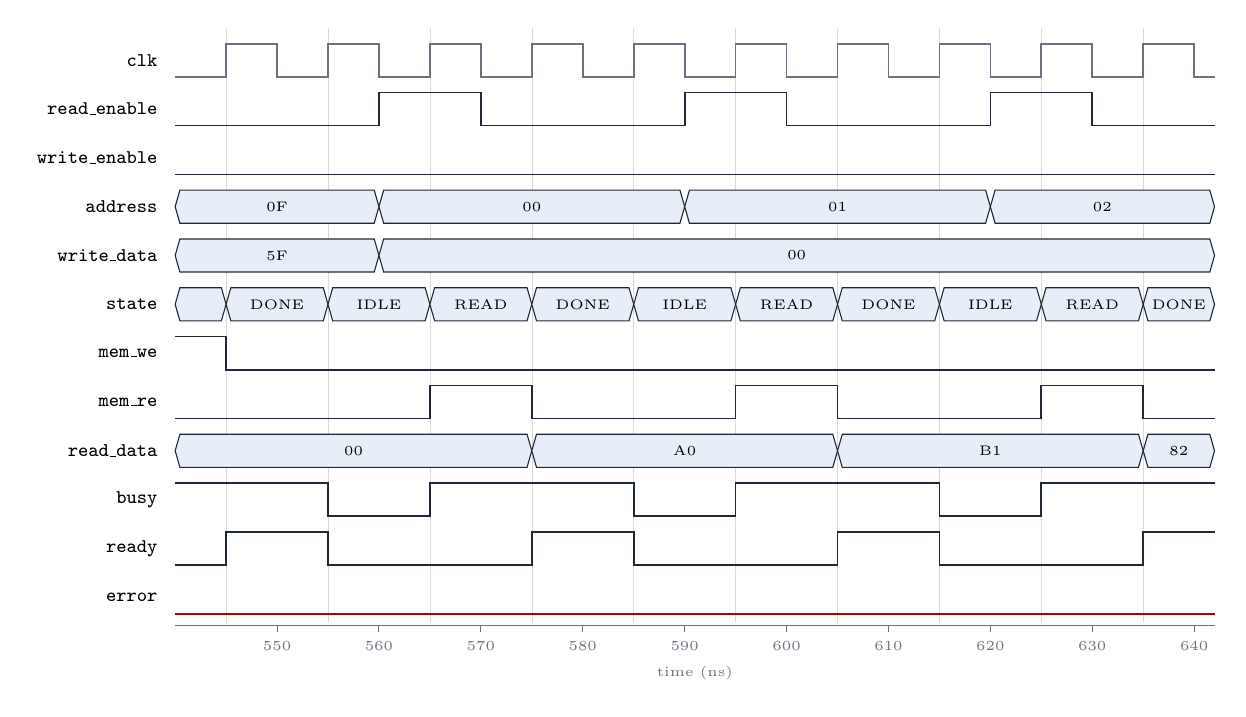
\begin{tikzpicture}[x=1cm,y=1cm,font=\scriptsize]
\draw[gray!30,very thin] (0.647,-0.1) -- (0.647,7.440);
\draw[gray!30,very thin] (1.941,-0.1) -- (1.941,7.440);
\draw[gray!30,very thin] (3.235,-0.1) -- (3.235,7.440);
\draw[gray!30,very thin] (4.529,-0.1) -- (4.529,7.440);
\draw[gray!30,very thin] (5.824,-0.1) -- (5.824,7.440);
\draw[gray!30,very thin] (7.118,-0.1) -- (7.118,7.440);
\draw[gray!30,very thin] (8.412,-0.1) -- (8.412,7.440);
\draw[gray!30,very thin] (9.706,-0.1) -- (9.706,7.440);
\draw[gray!30,very thin] (11.000,-0.1) -- (11.000,7.440);
\draw[gray!30,very thin] (12.294,-0.1) -- (12.294,7.440);
\node[anchor=east,font=\scriptsize\ttfamily] at (-0.1,7.030) {clk};
\draw[mut,line width=0.6pt] (0.000,6.820) -- (0.647,6.820) -- (0.647,7.240) -- (1.294,7.240) -- (1.294,6.820) -- (1.941,6.820) -- (1.941,7.240) -- (2.588,7.240) -- (2.588,6.820) -- (3.235,6.820) -- (3.235,7.240) -- (3.882,7.240) -- (3.882,6.820) -- (4.529,6.820) -- (4.529,7.240) -- (5.176,7.240) -- (5.176,6.820) -- (5.824,6.820) -- (5.824,7.240) -- (6.471,7.240) -- (6.471,6.820) -- (7.118,6.820) -- (7.118,7.240) -- (7.765,7.240) -- (7.765,6.820) -- (8.412,6.820) -- (8.412,7.240) -- (9.059,7.240) -- (9.059,6.820) -- (9.706,6.820) -- (9.706,7.240) -- (10.353,7.240) -- (10.353,6.820) -- (11.000,6.820) -- (11.000,7.240) -- (11.647,7.240) -- (11.647,6.820) -- (12.294,6.820) -- (12.294,7.240) -- (12.941,7.240) -- (12.941,6.820) -- (13.200,6.820);
\node[anchor=east,font=\scriptsize\ttfamily] at (-0.1,6.410) {read\_enable};
\draw[ink,line width=0.6pt] (0.000,6.200) -- (2.588,6.200) -- (2.588,6.620) -- (3.882,6.620) -- (3.882,6.200) -- (6.471,6.200) -- (6.471,6.620) -- (7.765,6.620) -- (7.765,6.200) -- (10.353,6.200) -- (10.353,6.620) -- (11.647,6.620) -- (11.647,6.200) -- (13.200,6.200);
\node[anchor=east,font=\scriptsize\ttfamily] at (-0.1,5.790) {write\_enable};
\draw[ink,line width=0.6pt] (0.000,5.580) -- (13.200,5.580);
\node[anchor=east,font=\scriptsize\ttfamily] at (-0.1,5.170) {address};
\draw[ink,fill=box,line width=0.4pt] (0.000,5.170) -- (0.060,4.960) -- (2.528,4.960) -- (2.588,5.170) -- (2.528,5.380) -- (0.060,5.380) -- cycle;
\node[font=\tiny] at (1.294,5.170) {0F};
\draw[ink,fill=box,line width=0.4pt] (2.588,5.170) -- (2.648,4.960) -- (6.411,4.960) -- (6.471,5.170) -- (6.411,5.380) -- (2.648,5.380) -- cycle;
\node[font=\tiny] at (4.529,5.170) {00};
\draw[ink,fill=box,line width=0.4pt] (6.471,5.170) -- (6.531,4.960) -- (10.293,4.960) -- (10.353,5.170) -- (10.293,5.380) -- (6.531,5.380) -- cycle;
\node[font=\tiny] at (8.412,5.170) {01};
\draw[ink,fill=box,line width=0.4pt] (10.353,5.170) -- (10.413,4.960) -- (13.140,4.960) -- (13.200,5.170) -- (13.140,5.380) -- (10.413,5.380) -- cycle;
\node[font=\tiny] at (11.776,5.170) {02};
\node[anchor=east,font=\scriptsize\ttfamily] at (-0.1,4.550) {write\_data};
\draw[ink,fill=box,line width=0.4pt] (0.000,4.550) -- (0.060,4.340) -- (2.528,4.340) -- (2.588,4.550) -- (2.528,4.760) -- (0.060,4.760) -- cycle;
\node[font=\tiny] at (1.294,4.550) {5F};
\draw[ink,fill=box,line width=0.4pt] (2.588,4.550) -- (2.648,4.340) -- (13.140,4.340) -- (13.200,4.550) -- (13.140,4.760) -- (2.648,4.760) -- cycle;
\node[font=\tiny] at (7.894,4.550) {00};
\node[anchor=east,font=\scriptsize\ttfamily] at (-0.1,3.930) {state};
\draw[ink,fill=box,line width=0.4pt] (0.000,3.930) -- (0.060,3.720) -- (0.587,3.720) -- (0.647,3.930) -- (0.587,4.140) -- (0.060,4.140) -- cycle;
\draw[ink,fill=box,line width=0.4pt] (0.647,3.930) -- (0.707,3.720) -- (1.881,3.720) -- (1.941,3.930) -- (1.881,4.140) -- (0.707,4.140) -- cycle;
\node[font=\tiny] at (1.294,3.930) {DONE};
\draw[ink,fill=box,line width=0.4pt] (1.941,3.930) -- (2.001,3.720) -- (3.175,3.720) -- (3.235,3.930) -- (3.175,4.140) -- (2.001,4.140) -- cycle;
\node[font=\tiny] at (2.588,3.930) {IDLE};
\draw[ink,fill=box,line width=0.4pt] (3.235,3.930) -- (3.295,3.720) -- (4.469,3.720) -- (4.529,3.930) -- (4.469,4.140) -- (3.295,4.140) -- cycle;
\node[font=\tiny] at (3.882,3.930) {READ};
\draw[ink,fill=box,line width=0.4pt] (4.529,3.930) -- (4.589,3.720) -- (5.764,3.720) -- (5.824,3.930) -- (5.764,4.140) -- (4.589,4.140) -- cycle;
\node[font=\tiny] at (5.176,3.930) {DONE};
\draw[ink,fill=box,line width=0.4pt] (5.824,3.930) -- (5.884,3.720) -- (7.058,3.720) -- (7.118,3.930) -- (7.058,4.140) -- (5.884,4.140) -- cycle;
\node[font=\tiny] at (6.471,3.930) {IDLE};
\draw[ink,fill=box,line width=0.4pt] (7.118,3.930) -- (7.178,3.720) -- (8.352,3.720) -- (8.412,3.930) -- (8.352,4.140) -- (7.178,4.140) -- cycle;
\node[font=\tiny] at (7.765,3.930) {READ};
\draw[ink,fill=box,line width=0.4pt] (8.412,3.930) -- (8.472,3.720) -- (9.646,3.720) -- (9.706,3.930) -- (9.646,4.140) -- (8.472,4.140) -- cycle;
\node[font=\tiny] at (9.059,3.930) {DONE};
\draw[ink,fill=box,line width=0.4pt] (9.706,3.930) -- (9.766,3.720) -- (10.940,3.720) -- (11.000,3.930) -- (10.940,4.140) -- (9.766,4.140) -- cycle;
\node[font=\tiny] at (10.353,3.930) {IDLE};
\draw[ink,fill=box,line width=0.4pt] (11.000,3.930) -- (11.060,3.720) -- (12.234,3.720) -- (12.294,3.930) -- (12.234,4.140) -- (11.060,4.140) -- cycle;
\node[font=\tiny] at (11.647,3.930) {READ};
\draw[ink,fill=box,line width=0.4pt] (12.294,3.930) -- (12.354,3.720) -- (13.140,3.720) -- (13.200,3.930) -- (13.140,4.140) -- (12.354,4.140) -- cycle;
\node[font=\tiny] at (12.747,3.930) {DONE};
\node[anchor=east,font=\scriptsize\ttfamily] at (-0.1,3.310) {mem\_we};
\draw[ink,line width=0.6pt] (0.000,3.520) -- (0.647,3.520) -- (0.647,3.100) -- (13.200,3.100);
\node[anchor=east,font=\scriptsize\ttfamily] at (-0.1,2.690) {mem\_re};
\draw[ink,line width=0.6pt] (0.000,2.480) -- (3.235,2.480) -- (3.235,2.900) -- (4.529,2.900) -- (4.529,2.480) -- (7.118,2.480) -- (7.118,2.900) -- (8.412,2.900) -- (8.412,2.480) -- (11.000,2.480) -- (11.000,2.900) -- (12.294,2.900) -- (12.294,2.480) -- (13.200,2.480);
\node[anchor=east,font=\scriptsize\ttfamily] at (-0.1,2.070) {read\_data};
\draw[ink,fill=box,line width=0.4pt] (0.000,2.070) -- (0.060,1.860) -- (4.469,1.860) -- (4.529,2.070) -- (4.469,2.280) -- (0.060,2.280) -- cycle;
\node[font=\tiny] at (2.265,2.070) {00};
\draw[ink,fill=box,line width=0.4pt] (4.529,2.070) -- (4.589,1.860) -- (8.352,1.860) -- (8.412,2.070) -- (8.352,2.280) -- (4.589,2.280) -- cycle;
\node[font=\tiny] at (6.471,2.070) {A0};
\draw[ink,fill=box,line width=0.4pt] (8.412,2.070) -- (8.472,1.860) -- (12.234,1.860) -- (12.294,2.070) -- (12.234,2.280) -- (8.472,2.280) -- cycle;
\node[font=\tiny] at (10.353,2.070) {B1};
\draw[ink,fill=box,line width=0.4pt] (12.294,2.070) -- (12.354,1.860) -- (13.140,1.860) -- (13.200,2.070) -- (13.140,2.280) -- (12.354,2.280) -- cycle;
\node[font=\tiny] at (12.747,2.070) {82};
\node[anchor=east,font=\scriptsize\ttfamily] at (-0.1,1.450) {busy};
\draw[ink,line width=0.6pt] (0.000,1.660) -- (1.941,1.660) -- (1.941,1.240) -- (3.235,1.240) -- (3.235,1.660) -- (5.824,1.660) -- (5.824,1.240) -- (7.118,1.240) -- (7.118,1.660) -- (9.706,1.660) -- (9.706,1.240) -- (11.000,1.240) -- (11.000,1.660) -- (13.200,1.660);
\node[anchor=east,font=\scriptsize\ttfamily] at (-0.1,0.830) {ready};
\draw[ink,line width=0.6pt] (0.000,0.620) -- (0.647,0.620) -- (0.647,1.040) -- (1.941,1.040) -- (1.941,0.620) -- (4.529,0.620) -- (4.529,1.040) -- (5.824,1.040) -- (5.824,0.620) -- (8.412,0.620) -- (8.412,1.040) -- (9.706,1.040) -- (9.706,0.620) -- (12.294,0.620) -- (12.294,1.040) -- (13.200,1.040);
\node[anchor=east,font=\scriptsize\ttfamily] at (-0.1,0.210) {error};
\draw[red!70!black,line width=0.6pt] (0.000,0.000) -- (13.200,0.000);
\draw[mut] (0,-0.15) -- (13.200,-0.15);
\draw[mut] (1.294,-0.15) -- ++(0,-0.08) node[below,font=\tiny,text=mut] {550};
\draw[mut] (2.588,-0.15) -- ++(0,-0.08) node[below,font=\tiny,text=mut] {560};
\draw[mut] (3.882,-0.15) -- ++(0,-0.08) node[below,font=\tiny,text=mut] {570};
\draw[mut] (5.176,-0.15) -- ++(0,-0.08) node[below,font=\tiny,text=mut] {580};
\draw[mut] (6.471,-0.15) -- ++(0,-0.08) node[below,font=\tiny,text=mut] {590};
\draw[mut] (7.765,-0.15) -- ++(0,-0.08) node[below,font=\tiny,text=mut] {600};
\draw[mut] (9.059,-0.15) -- ++(0,-0.08) node[below,font=\tiny,text=mut] {610};
\draw[mut] (10.353,-0.15) -- ++(0,-0.08) node[below,font=\tiny,text=mut] {620};
\draw[mut] (11.647,-0.15) -- ++(0,-0.08) node[below,font=\tiny,text=mut] {630};
\draw[mut] (12.941,-0.15) -- ++(0,-0.08) node[below,font=\tiny,text=mut] {640};
\node[font=\tiny,text=mut] at (6.600,-0.75) {time (ns)};
\end{tikzpicture}}
\caption{Back-to-back reads with zero wait states}
\label{fig:r0}
\end{figure}
\sig{mem\_re} is high during READ; the registered memory output updates on the edge that ends READ, so \sig{read\_data} already holds the addressed word when \sig{ready} is high in DONE, and it stays stable afterwards.

\begin{figure}[H]
\centering
\resizebox{\textwidth}{!}{%
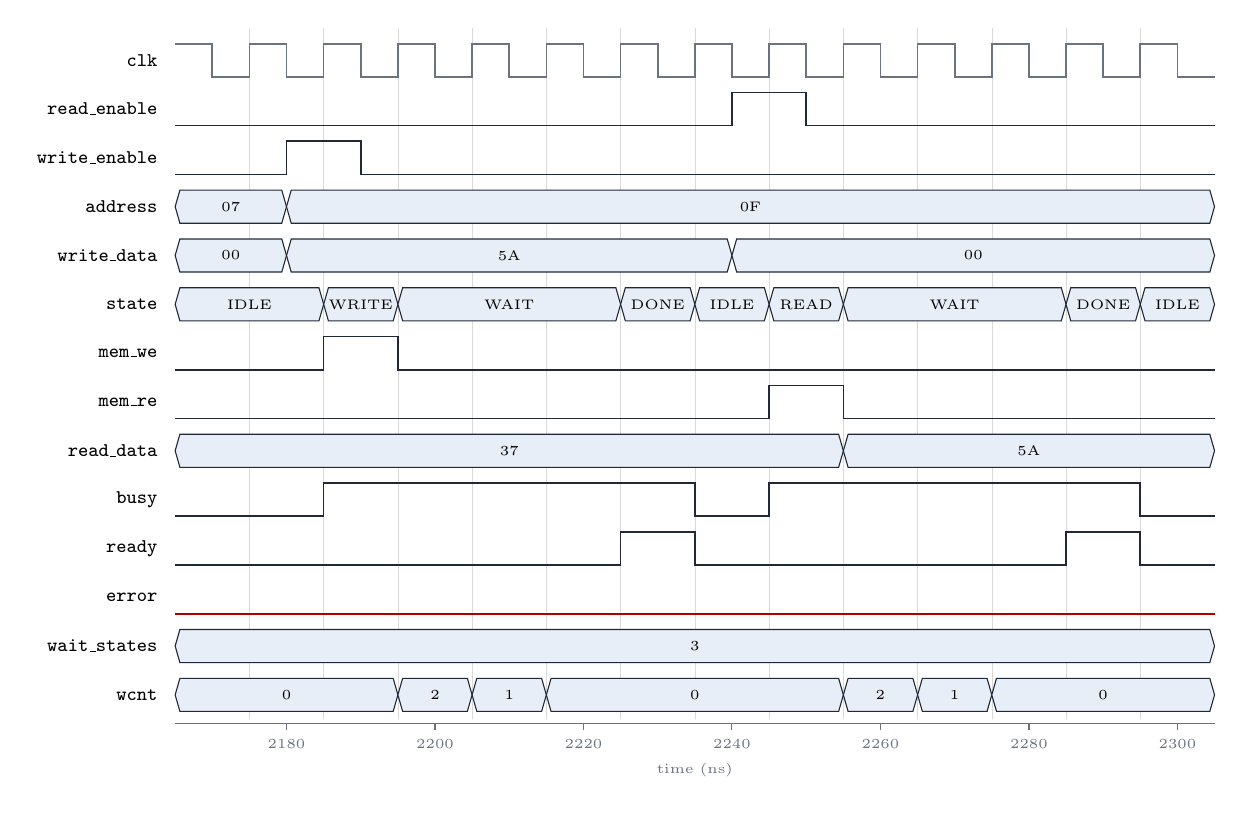
\begin{tikzpicture}[x=1cm,y=1cm,font=\scriptsize]
\draw[gray!30,very thin] (0.943,-0.1) -- (0.943,8.680);
\draw[gray!30,very thin] (1.886,-0.1) -- (1.886,8.680);
\draw[gray!30,very thin] (2.829,-0.1) -- (2.829,8.680);
\draw[gray!30,very thin] (3.771,-0.1) -- (3.771,8.680);
\draw[gray!30,very thin] (4.714,-0.1) -- (4.714,8.680);
\draw[gray!30,very thin] (5.657,-0.1) -- (5.657,8.680);
\draw[gray!30,very thin] (6.600,-0.1) -- (6.600,8.680);
\draw[gray!30,very thin] (7.543,-0.1) -- (7.543,8.680);
\draw[gray!30,very thin] (8.486,-0.1) -- (8.486,8.680);
\draw[gray!30,very thin] (9.429,-0.1) -- (9.429,8.680);
\draw[gray!30,very thin] (10.371,-0.1) -- (10.371,8.680);
\draw[gray!30,very thin] (11.314,-0.1) -- (11.314,8.680);
\draw[gray!30,very thin] (12.257,-0.1) -- (12.257,8.680);
\node[anchor=east,font=\scriptsize\ttfamily] at (-0.1,8.270) {clk};
\draw[mut,line width=0.6pt] (0.000,8.480) -- (0.471,8.480) -- (0.471,8.060) -- (0.943,8.060) -- (0.943,8.480) -- (1.414,8.480) -- (1.414,8.060) -- (1.886,8.060) -- (1.886,8.480) -- (2.357,8.480) -- (2.357,8.060) -- (2.829,8.060) -- (2.829,8.480) -- (3.300,8.480) -- (3.300,8.060) -- (3.771,8.060) -- (3.771,8.480) -- (4.243,8.480) -- (4.243,8.060) -- (4.714,8.060) -- (4.714,8.480) -- (5.186,8.480) -- (5.186,8.060) -- (5.657,8.060) -- (5.657,8.480) -- (6.129,8.480) -- (6.129,8.060) -- (6.600,8.060) -- (6.600,8.480) -- (7.071,8.480) -- (7.071,8.060) -- (7.543,8.060) -- (7.543,8.480) -- (8.014,8.480) -- (8.014,8.060) -- (8.486,8.060) -- (8.486,8.480) -- (8.957,8.480) -- (8.957,8.060) -- (9.429,8.060) -- (9.429,8.480) -- (9.900,8.480) -- (9.900,8.060) -- (10.371,8.060) -- (10.371,8.480) -- (10.843,8.480) -- (10.843,8.060) -- (11.314,8.060) -- (11.314,8.480) -- (11.786,8.480) -- (11.786,8.060) -- (12.257,8.060) -- (12.257,8.480) -- (12.729,8.480) -- (12.729,8.060) -- (13.200,8.060);
\node[anchor=east,font=\scriptsize\ttfamily] at (-0.1,7.650) {read\_enable};
\draw[ink,line width=0.6pt] (0.000,7.440) -- (7.071,7.440) -- (7.071,7.860) -- (8.014,7.860) -- (8.014,7.440) -- (13.200,7.440);
\node[anchor=east,font=\scriptsize\ttfamily] at (-0.1,7.030) {write\_enable};
\draw[ink,line width=0.6pt] (0.000,6.820) -- (1.414,6.820) -- (1.414,7.240) -- (2.357,7.240) -- (2.357,6.820) -- (13.200,6.820);
\node[anchor=east,font=\scriptsize\ttfamily] at (-0.1,6.410) {address};
\draw[ink,fill=box,line width=0.4pt] (0.000,6.410) -- (0.060,6.200) -- (1.354,6.200) -- (1.414,6.410) -- (1.354,6.620) -- (0.060,6.620) -- cycle;
\node[font=\tiny] at (0.707,6.410) {07};
\draw[ink,fill=box,line width=0.4pt] (1.414,6.410) -- (1.474,6.200) -- (13.140,6.200) -- (13.200,6.410) -- (13.140,6.620) -- (1.474,6.620) -- cycle;
\node[font=\tiny] at (7.307,6.410) {0F};
\node[anchor=east,font=\scriptsize\ttfamily] at (-0.1,5.790) {write\_data};
\draw[ink,fill=box,line width=0.4pt] (0.000,5.790) -- (0.060,5.580) -- (1.354,5.580) -- (1.414,5.790) -- (1.354,6.000) -- (0.060,6.000) -- cycle;
\node[font=\tiny] at (0.707,5.790) {00};
\draw[ink,fill=box,line width=0.4pt] (1.414,5.790) -- (1.474,5.580) -- (7.011,5.580) -- (7.071,5.790) -- (7.011,6.000) -- (1.474,6.000) -- cycle;
\node[font=\tiny] at (4.243,5.790) {5A};
\draw[ink,fill=box,line width=0.4pt] (7.071,5.790) -- (7.131,5.580) -- (13.140,5.580) -- (13.200,5.790) -- (13.140,6.000) -- (7.131,6.000) -- cycle;
\node[font=\tiny] at (10.136,5.790) {00};
\node[anchor=east,font=\scriptsize\ttfamily] at (-0.1,5.170) {state};
\draw[ink,fill=box,line width=0.4pt] (0.000,5.170) -- (0.060,4.960) -- (1.826,4.960) -- (1.886,5.170) -- (1.826,5.380) -- (0.060,5.380) -- cycle;
\node[font=\tiny] at (0.943,5.170) {IDLE};
\draw[ink,fill=box,line width=0.4pt] (1.886,5.170) -- (1.946,4.960) -- (2.769,4.960) -- (2.829,5.170) -- (2.769,5.380) -- (1.946,5.380) -- cycle;
\node[font=\tiny] at (2.357,5.170) {WRITE};
\draw[ink,fill=box,line width=0.4pt] (2.829,5.170) -- (2.889,4.960) -- (5.597,4.960) -- (5.657,5.170) -- (5.597,5.380) -- (2.889,5.380) -- cycle;
\node[font=\tiny] at (4.243,5.170) {WAIT};
\draw[ink,fill=box,line width=0.4pt] (5.657,5.170) -- (5.717,4.960) -- (6.540,4.960) -- (6.600,5.170) -- (6.540,5.380) -- (5.717,5.380) -- cycle;
\node[font=\tiny] at (6.129,5.170) {DONE};
\draw[ink,fill=box,line width=0.4pt] (6.600,5.170) -- (6.660,4.960) -- (7.483,4.960) -- (7.543,5.170) -- (7.483,5.380) -- (6.660,5.380) -- cycle;
\node[font=\tiny] at (7.071,5.170) {IDLE};
\draw[ink,fill=box,line width=0.4pt] (7.543,5.170) -- (7.603,4.960) -- (8.426,4.960) -- (8.486,5.170) -- (8.426,5.380) -- (7.603,5.380) -- cycle;
\node[font=\tiny] at (8.014,5.170) {READ};
\draw[ink,fill=box,line width=0.4pt] (8.486,5.170) -- (8.546,4.960) -- (11.254,4.960) -- (11.314,5.170) -- (11.254,5.380) -- (8.546,5.380) -- cycle;
\node[font=\tiny] at (9.900,5.170) {WAIT};
\draw[ink,fill=box,line width=0.4pt] (11.314,5.170) -- (11.374,4.960) -- (12.197,4.960) -- (12.257,5.170) -- (12.197,5.380) -- (11.374,5.380) -- cycle;
\node[font=\tiny] at (11.786,5.170) {DONE};
\draw[ink,fill=box,line width=0.4pt] (12.257,5.170) -- (12.317,4.960) -- (13.140,4.960) -- (13.200,5.170) -- (13.140,5.380) -- (12.317,5.380) -- cycle;
\node[font=\tiny] at (12.729,5.170) {IDLE};
\node[anchor=east,font=\scriptsize\ttfamily] at (-0.1,4.550) {mem\_we};
\draw[ink,line width=0.6pt] (0.000,4.340) -- (1.886,4.340) -- (1.886,4.760) -- (2.829,4.760) -- (2.829,4.340) -- (13.200,4.340);
\node[anchor=east,font=\scriptsize\ttfamily] at (-0.1,3.930) {mem\_re};
\draw[ink,line width=0.6pt] (0.000,3.720) -- (7.543,3.720) -- (7.543,4.140) -- (8.486,4.140) -- (8.486,3.720) -- (13.200,3.720);
\node[anchor=east,font=\scriptsize\ttfamily] at (-0.1,3.310) {read\_data};
\draw[ink,fill=box,line width=0.4pt] (0.000,3.310) -- (0.060,3.100) -- (8.426,3.100) -- (8.486,3.310) -- (8.426,3.520) -- (0.060,3.520) -- cycle;
\node[font=\tiny] at (4.243,3.310) {37};
\draw[ink,fill=box,line width=0.4pt] (8.486,3.310) -- (8.546,3.100) -- (13.140,3.100) -- (13.200,3.310) -- (13.140,3.520) -- (8.546,3.520) -- cycle;
\node[font=\tiny] at (10.843,3.310) {5A};
\node[anchor=east,font=\scriptsize\ttfamily] at (-0.1,2.690) {busy};
\draw[ink,line width=0.6pt] (0.000,2.480) -- (1.886,2.480) -- (1.886,2.900) -- (6.600,2.900) -- (6.600,2.480) -- (7.543,2.480) -- (7.543,2.900) -- (12.257,2.900) -- (12.257,2.480) -- (13.200,2.480);
\node[anchor=east,font=\scriptsize\ttfamily] at (-0.1,2.070) {ready};
\draw[ink,line width=0.6pt] (0.000,1.860) -- (5.657,1.860) -- (5.657,2.280) -- (6.600,2.280) -- (6.600,1.860) -- (11.314,1.860) -- (11.314,2.280) -- (12.257,2.280) -- (12.257,1.860) -- (13.200,1.860);
\node[anchor=east,font=\scriptsize\ttfamily] at (-0.1,1.450) {error};
\draw[red!70!black,line width=0.6pt] (0.000,1.240) -- (13.200,1.240);
\node[anchor=east,font=\scriptsize\ttfamily] at (-0.1,0.830) {wait\_states};
\draw[ink,fill=box,line width=0.4pt] (0.000,0.830) -- (0.060,0.620) -- (13.140,0.620) -- (13.200,0.830) -- (13.140,1.040) -- (0.060,1.040) -- cycle;
\node[font=\tiny] at (6.600,0.830) {3};
\node[anchor=east,font=\scriptsize\ttfamily] at (-0.1,0.210) {wcnt};
\draw[ink,fill=box,line width=0.4pt] (0.000,0.210) -- (0.060,0.000) -- (2.769,0.000) -- (2.829,0.210) -- (2.769,0.420) -- (0.060,0.420) -- cycle;
\node[font=\tiny] at (1.414,0.210) {0};
\draw[ink,fill=box,line width=0.4pt] (2.829,0.210) -- (2.889,0.000) -- (3.711,0.000) -- (3.771,0.210) -- (3.711,0.420) -- (2.889,0.420) -- cycle;
\node[font=\tiny] at (3.300,0.210) {2};
\draw[ink,fill=box,line width=0.4pt] (3.771,0.210) -- (3.831,0.000) -- (4.654,0.000) -- (4.714,0.210) -- (4.654,0.420) -- (3.831,0.420) -- cycle;
\node[font=\tiny] at (4.243,0.210) {1};
\draw[ink,fill=box,line width=0.4pt] (4.714,0.210) -- (4.774,0.000) -- (8.426,0.000) -- (8.486,0.210) -- (8.426,0.420) -- (4.774,0.420) -- cycle;
\node[font=\tiny] at (6.600,0.210) {0};
\draw[ink,fill=box,line width=0.4pt] (8.486,0.210) -- (8.546,0.000) -- (9.369,0.000) -- (9.429,0.210) -- (9.369,0.420) -- (8.546,0.420) -- cycle;
\node[font=\tiny] at (8.957,0.210) {2};
\draw[ink,fill=box,line width=0.4pt] (9.429,0.210) -- (9.489,0.000) -- (10.311,0.000) -- (10.371,0.210) -- (10.311,0.420) -- (9.489,0.420) -- cycle;
\node[font=\tiny] at (9.900,0.210) {1};
\draw[ink,fill=box,line width=0.4pt] (10.371,0.210) -- (10.431,0.000) -- (13.140,0.000) -- (13.200,0.210) -- (13.140,0.420) -- (10.431,0.420) -- cycle;
\node[font=\tiny] at (11.786,0.210) {0};
\draw[mut] (0,-0.15) -- (13.200,-0.15);
\draw[mut] (1.414,-0.15) -- ++(0,-0.08) node[below,font=\tiny,text=mut] {2180};
\draw[mut] (3.300,-0.15) -- ++(0,-0.08) node[below,font=\tiny,text=mut] {2200};
\draw[mut] (5.186,-0.15) -- ++(0,-0.08) node[below,font=\tiny,text=mut] {2220};
\draw[mut] (7.071,-0.15) -- ++(0,-0.08) node[below,font=\tiny,text=mut] {2240};
\draw[mut] (8.957,-0.15) -- ++(0,-0.08) node[below,font=\tiny,text=mut] {2260};
\draw[mut] (10.843,-0.15) -- ++(0,-0.08) node[below,font=\tiny,text=mut] {2280};
\draw[mut] (12.729,-0.15) -- ++(0,-0.08) node[below,font=\tiny,text=mut] {2300};
\node[font=\tiny,text=mut] at (6.600,-0.75) {time (ns)};
\end{tikzpicture}}
\caption{Write and read of address 0xF with three programmed wait states}
\label{fig:w3}
\end{figure}
With WAIT = 3 the FSM passes through WAIT for exactly three cycles while \sig{wcnt} counts 2, 1, 0. Latency grows from 2 to 5 cycles and \sig{busy} remains high for the whole transaction. The read returns 0x5A, the value written just before.

\begin{figure}[H]
\centering
\resizebox{\textwidth}{!}{%
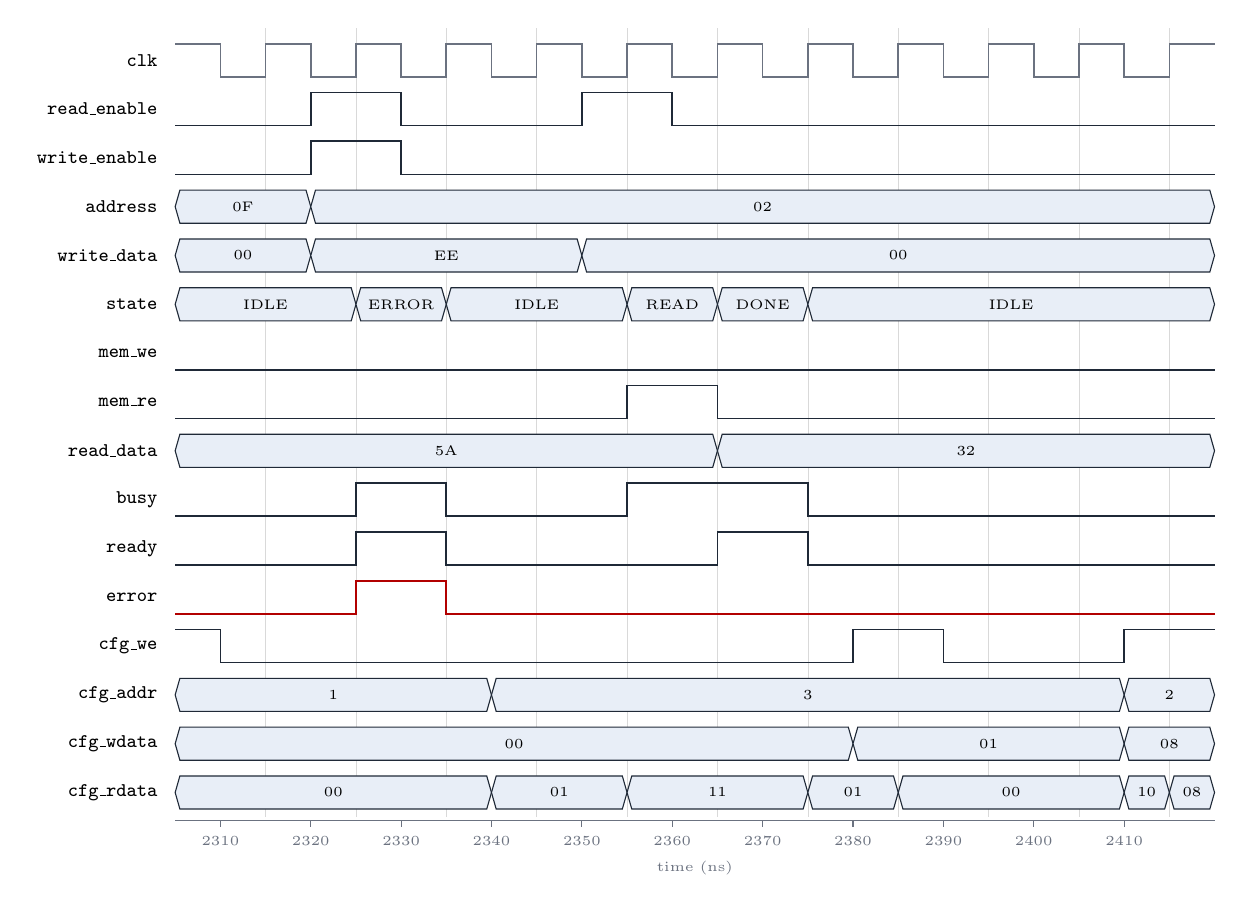
\begin{tikzpicture}[x=1cm,y=1cm,font=\scriptsize]
\draw[gray!30,very thin] (1.148,-0.1) -- (1.148,9.920);
\draw[gray!30,very thin] (2.296,-0.1) -- (2.296,9.920);
\draw[gray!30,very thin] (3.443,-0.1) -- (3.443,9.920);
\draw[gray!30,very thin] (4.591,-0.1) -- (4.591,9.920);
\draw[gray!30,very thin] (5.739,-0.1) -- (5.739,9.920);
\draw[gray!30,very thin] (6.887,-0.1) -- (6.887,9.920);
\draw[gray!30,very thin] (8.035,-0.1) -- (8.035,9.920);
\draw[gray!30,very thin] (9.183,-0.1) -- (9.183,9.920);
\draw[gray!30,very thin] (10.330,-0.1) -- (10.330,9.920);
\draw[gray!30,very thin] (11.478,-0.1) -- (11.478,9.920);
\draw[gray!30,very thin] (12.626,-0.1) -- (12.626,9.920);
\node[anchor=east,font=\scriptsize\ttfamily] at (-0.1,9.510) {clk};
\draw[mut,line width=0.6pt] (0.000,9.720) -- (0.574,9.720) -- (0.574,9.300) -- (1.148,9.300) -- (1.148,9.720) -- (1.722,9.720) -- (1.722,9.300) -- (2.296,9.300) -- (2.296,9.720) -- (2.870,9.720) -- (2.870,9.300) -- (3.443,9.300) -- (3.443,9.720) -- (4.017,9.720) -- (4.017,9.300) -- (4.591,9.300) -- (4.591,9.720) -- (5.165,9.720) -- (5.165,9.300) -- (5.739,9.300) -- (5.739,9.720) -- (6.313,9.720) -- (6.313,9.300) -- (6.887,9.300) -- (6.887,9.720) -- (7.461,9.720) -- (7.461,9.300) -- (8.035,9.300) -- (8.035,9.720) -- (8.609,9.720) -- (8.609,9.300) -- (9.183,9.300) -- (9.183,9.720) -- (9.757,9.720) -- (9.757,9.300) -- (10.330,9.300) -- (10.330,9.720) -- (10.904,9.720) -- (10.904,9.300) -- (11.478,9.300) -- (11.478,9.720) -- (12.052,9.720) -- (12.052,9.300) -- (12.626,9.300) -- (12.626,9.720) -- (13.200,9.720);
\node[anchor=east,font=\scriptsize\ttfamily] at (-0.1,8.890) {read\_enable};
\draw[ink,line width=0.6pt] (0.000,8.680) -- (1.722,8.680) -- (1.722,9.100) -- (2.870,9.100) -- (2.870,8.680) -- (5.165,8.680) -- (5.165,9.100) -- (6.313,9.100) -- (6.313,8.680) -- (13.200,8.680);
\node[anchor=east,font=\scriptsize\ttfamily] at (-0.1,8.270) {write\_enable};
\draw[ink,line width=0.6pt] (0.000,8.060) -- (1.722,8.060) -- (1.722,8.480) -- (2.870,8.480) -- (2.870,8.060) -- (13.200,8.060);
\node[anchor=east,font=\scriptsize\ttfamily] at (-0.1,7.650) {address};
\draw[ink,fill=box,line width=0.4pt] (0.000,7.650) -- (0.060,7.440) -- (1.662,7.440) -- (1.722,7.650) -- (1.662,7.860) -- (0.060,7.860) -- cycle;
\node[font=\tiny] at (0.861,7.650) {0F};
\draw[ink,fill=box,line width=0.4pt] (1.722,7.650) -- (1.782,7.440) -- (13.140,7.440) -- (13.200,7.650) -- (13.140,7.860) -- (1.782,7.860) -- cycle;
\node[font=\tiny] at (7.461,7.650) {02};
\node[anchor=east,font=\scriptsize\ttfamily] at (-0.1,7.030) {write\_data};
\draw[ink,fill=box,line width=0.4pt] (0.000,7.030) -- (0.060,6.820) -- (1.662,6.820) -- (1.722,7.030) -- (1.662,7.240) -- (0.060,7.240) -- cycle;
\node[font=\tiny] at (0.861,7.030) {00};
\draw[ink,fill=box,line width=0.4pt] (1.722,7.030) -- (1.782,6.820) -- (5.105,6.820) -- (5.165,7.030) -- (5.105,7.240) -- (1.782,7.240) -- cycle;
\node[font=\tiny] at (3.443,7.030) {EE};
\draw[ink,fill=box,line width=0.4pt] (5.165,7.030) -- (5.225,6.820) -- (13.140,6.820) -- (13.200,7.030) -- (13.140,7.240) -- (5.225,7.240) -- cycle;
\node[font=\tiny] at (9.183,7.030) {00};
\node[anchor=east,font=\scriptsize\ttfamily] at (-0.1,6.410) {state};
\draw[ink,fill=box,line width=0.4pt] (0.000,6.410) -- (0.060,6.200) -- (2.236,6.200) -- (2.296,6.410) -- (2.236,6.620) -- (0.060,6.620) -- cycle;
\node[font=\tiny] at (1.148,6.410) {IDLE};
\draw[ink,fill=box,line width=0.4pt] (2.296,6.410) -- (2.356,6.200) -- (3.383,6.200) -- (3.443,6.410) -- (3.383,6.620) -- (2.356,6.620) -- cycle;
\node[font=\tiny] at (2.870,6.410) {ERROR};
\draw[ink,fill=box,line width=0.4pt] (3.443,6.410) -- (3.503,6.200) -- (5.679,6.200) -- (5.739,6.410) -- (5.679,6.620) -- (3.503,6.620) -- cycle;
\node[font=\tiny] at (4.591,6.410) {IDLE};
\draw[ink,fill=box,line width=0.4pt] (5.739,6.410) -- (5.799,6.200) -- (6.827,6.200) -- (6.887,6.410) -- (6.827,6.620) -- (5.799,6.620) -- cycle;
\node[font=\tiny] at (6.313,6.410) {READ};
\draw[ink,fill=box,line width=0.4pt] (6.887,6.410) -- (6.947,6.200) -- (7.975,6.200) -- (8.035,6.410) -- (7.975,6.620) -- (6.947,6.620) -- cycle;
\node[font=\tiny] at (7.461,6.410) {DONE};
\draw[ink,fill=box,line width=0.4pt] (8.035,6.410) -- (8.095,6.200) -- (13.140,6.200) -- (13.200,6.410) -- (13.140,6.620) -- (8.095,6.620) -- cycle;
\node[font=\tiny] at (10.617,6.410) {IDLE};
\node[anchor=east,font=\scriptsize\ttfamily] at (-0.1,5.790) {mem\_we};
\draw[ink,line width=0.6pt] (0.000,5.580) -- (13.200,5.580);
\node[anchor=east,font=\scriptsize\ttfamily] at (-0.1,5.170) {mem\_re};
\draw[ink,line width=0.6pt] (0.000,4.960) -- (5.739,4.960) -- (5.739,5.380) -- (6.887,5.380) -- (6.887,4.960) -- (13.200,4.960);
\node[anchor=east,font=\scriptsize\ttfamily] at (-0.1,4.550) {read\_data};
\draw[ink,fill=box,line width=0.4pt] (0.000,4.550) -- (0.060,4.340) -- (6.827,4.340) -- (6.887,4.550) -- (6.827,4.760) -- (0.060,4.760) -- cycle;
\node[font=\tiny] at (3.443,4.550) {5A};
\draw[ink,fill=box,line width=0.4pt] (6.887,4.550) -- (6.947,4.340) -- (13.140,4.340) -- (13.200,4.550) -- (13.140,4.760) -- (6.947,4.760) -- cycle;
\node[font=\tiny] at (10.043,4.550) {32};
\node[anchor=east,font=\scriptsize\ttfamily] at (-0.1,3.930) {busy};
\draw[ink,line width=0.6pt] (0.000,3.720) -- (2.296,3.720) -- (2.296,4.140) -- (3.443,4.140) -- (3.443,3.720) -- (5.739,3.720) -- (5.739,4.140) -- (8.035,4.140) -- (8.035,3.720) -- (13.200,3.720);
\node[anchor=east,font=\scriptsize\ttfamily] at (-0.1,3.310) {ready};
\draw[ink,line width=0.6pt] (0.000,3.100) -- (2.296,3.100) -- (2.296,3.520) -- (3.443,3.520) -- (3.443,3.100) -- (6.887,3.100) -- (6.887,3.520) -- (8.035,3.520) -- (8.035,3.100) -- (13.200,3.100);
\node[anchor=east,font=\scriptsize\ttfamily] at (-0.1,2.690) {error};
\draw[red!70!black,line width=0.6pt] (0.000,2.480) -- (2.296,2.480) -- (2.296,2.900) -- (3.443,2.900) -- (3.443,2.480) -- (13.200,2.480);
\node[anchor=east,font=\scriptsize\ttfamily] at (-0.1,2.070) {cfg\_we};
\draw[ink,line width=0.6pt] (0.000,2.280) -- (0.574,2.280) -- (0.574,1.860) -- (8.609,1.860) -- (8.609,2.280) -- (9.757,2.280) -- (9.757,1.860) -- (12.052,1.860) -- (12.052,2.280) -- (13.200,2.280);
\node[anchor=east,font=\scriptsize\ttfamily] at (-0.1,1.450) {cfg\_addr};
\draw[ink,fill=box,line width=0.4pt] (0.000,1.450) -- (0.060,1.240) -- (3.957,1.240) -- (4.017,1.450) -- (3.957,1.660) -- (0.060,1.660) -- cycle;
\node[font=\tiny] at (2.009,1.450) {1};
\draw[ink,fill=box,line width=0.4pt] (4.017,1.450) -- (4.077,1.240) -- (11.992,1.240) -- (12.052,1.450) -- (11.992,1.660) -- (4.077,1.660) -- cycle;
\node[font=\tiny] at (8.035,1.450) {3};
\draw[ink,fill=box,line width=0.4pt] (12.052,1.450) -- (12.112,1.240) -- (13.140,1.240) -- (13.200,1.450) -- (13.140,1.660) -- (12.112,1.660) -- cycle;
\node[font=\tiny] at (12.626,1.450) {2};
\node[anchor=east,font=\scriptsize\ttfamily] at (-0.1,0.830) {cfg\_wdata};
\draw[ink,fill=box,line width=0.4pt] (0.000,0.830) -- (0.060,0.620) -- (8.549,0.620) -- (8.609,0.830) -- (8.549,1.040) -- (0.060,1.040) -- cycle;
\node[font=\tiny] at (4.304,0.830) {00};
\draw[ink,fill=box,line width=0.4pt] (8.609,0.830) -- (8.669,0.620) -- (11.992,0.620) -- (12.052,0.830) -- (11.992,1.040) -- (8.669,1.040) -- cycle;
\node[font=\tiny] at (10.330,0.830) {01};
\draw[ink,fill=box,line width=0.4pt] (12.052,0.830) -- (12.112,0.620) -- (13.140,0.620) -- (13.200,0.830) -- (13.140,1.040) -- (12.112,1.040) -- cycle;
\node[font=\tiny] at (12.626,0.830) {08};
\node[anchor=east,font=\scriptsize\ttfamily] at (-0.1,0.210) {cfg\_rdata};
\draw[ink,fill=box,line width=0.4pt] (0.000,0.210) -- (0.060,0.000) -- (3.957,0.000) -- (4.017,0.210) -- (3.957,0.420) -- (0.060,0.420) -- cycle;
\node[font=\tiny] at (2.009,0.210) {00};
\draw[ink,fill=box,line width=0.4pt] (4.017,0.210) -- (4.077,0.000) -- (5.679,0.000) -- (5.739,0.210) -- (5.679,0.420) -- (4.077,0.420) -- cycle;
\node[font=\tiny] at (4.878,0.210) {01};
\draw[ink,fill=box,line width=0.4pt] (5.739,0.210) -- (5.799,0.000) -- (7.975,0.000) -- (8.035,0.210) -- (7.975,0.420) -- (5.799,0.420) -- cycle;
\node[font=\tiny] at (6.887,0.210) {11};
\draw[ink,fill=box,line width=0.4pt] (8.035,0.210) -- (8.095,0.000) -- (9.123,0.000) -- (9.183,0.210) -- (9.123,0.420) -- (8.095,0.420) -- cycle;
\node[font=\tiny] at (8.609,0.210) {01};
\draw[ink,fill=box,line width=0.4pt] (9.183,0.210) -- (9.243,0.000) -- (11.992,0.000) -- (12.052,0.210) -- (11.992,0.420) -- (9.243,0.420) -- cycle;
\node[font=\tiny] at (10.617,0.210) {00};
\draw[ink,fill=box,line width=0.4pt] (12.052,0.210) -- (12.112,0.000) -- (12.566,0.000) -- (12.626,0.210) -- (12.566,0.420) -- (12.112,0.420) -- cycle;
\node[font=\tiny] at (12.339,0.210) {10};
\draw[ink,fill=box,line width=0.4pt] (12.626,0.210) -- (12.686,0.000) -- (13.140,0.000) -- (13.200,0.210) -- (13.140,0.420) -- (12.686,0.420) -- cycle;
\node[font=\tiny] at (12.913,0.210) {08};
\draw[mut] (0,-0.15) -- (13.200,-0.15);
\draw[mut] (0.574,-0.15) -- ++(0,-0.08) node[below,font=\tiny,text=mut] {2310};
\draw[mut] (1.722,-0.15) -- ++(0,-0.08) node[below,font=\tiny,text=mut] {2320};
\draw[mut] (2.870,-0.15) -- ++(0,-0.08) node[below,font=\tiny,text=mut] {2330};
\draw[mut] (4.017,-0.15) -- ++(0,-0.08) node[below,font=\tiny,text=mut] {2340};
\draw[mut] (5.165,-0.15) -- ++(0,-0.08) node[below,font=\tiny,text=mut] {2350};
\draw[mut] (6.313,-0.15) -- ++(0,-0.08) node[below,font=\tiny,text=mut] {2360};
\draw[mut] (7.461,-0.15) -- ++(0,-0.08) node[below,font=\tiny,text=mut] {2370};
\draw[mut] (8.609,-0.15) -- ++(0,-0.08) node[below,font=\tiny,text=mut] {2380};
\draw[mut] (9.757,-0.15) -- ++(0,-0.08) node[below,font=\tiny,text=mut] {2390};
\draw[mut] (10.904,-0.15) -- ++(0,-0.08) node[below,font=\tiny,text=mut] {2400};
\draw[mut] (12.052,-0.15) -- ++(0,-0.08) node[below,font=\tiny,text=mut] {2410};
\node[font=\tiny,text=mut] at (6.600,-0.75) {time (ns)};
\end{tikzpicture}}
\caption{Simultaneous read and write request rejected}
\label{fig:coll}
\end{figure}
Both enables are high in the same cycle, so the FSM goes to ERROR instead of READ or WRITE. \sig{error} and \sig{ready} pulse together, neither \sig{mem\_we} nor \sig{mem\_re} is asserted, and a STATUS read-back returns 0x01 (COLL). The following read of address 0x2 confirms that memory is unchanged, and writing 0x01 to STATUS clears the bit.

\begin{figure}[H]
\centering
\resizebox{\textwidth}{!}{%
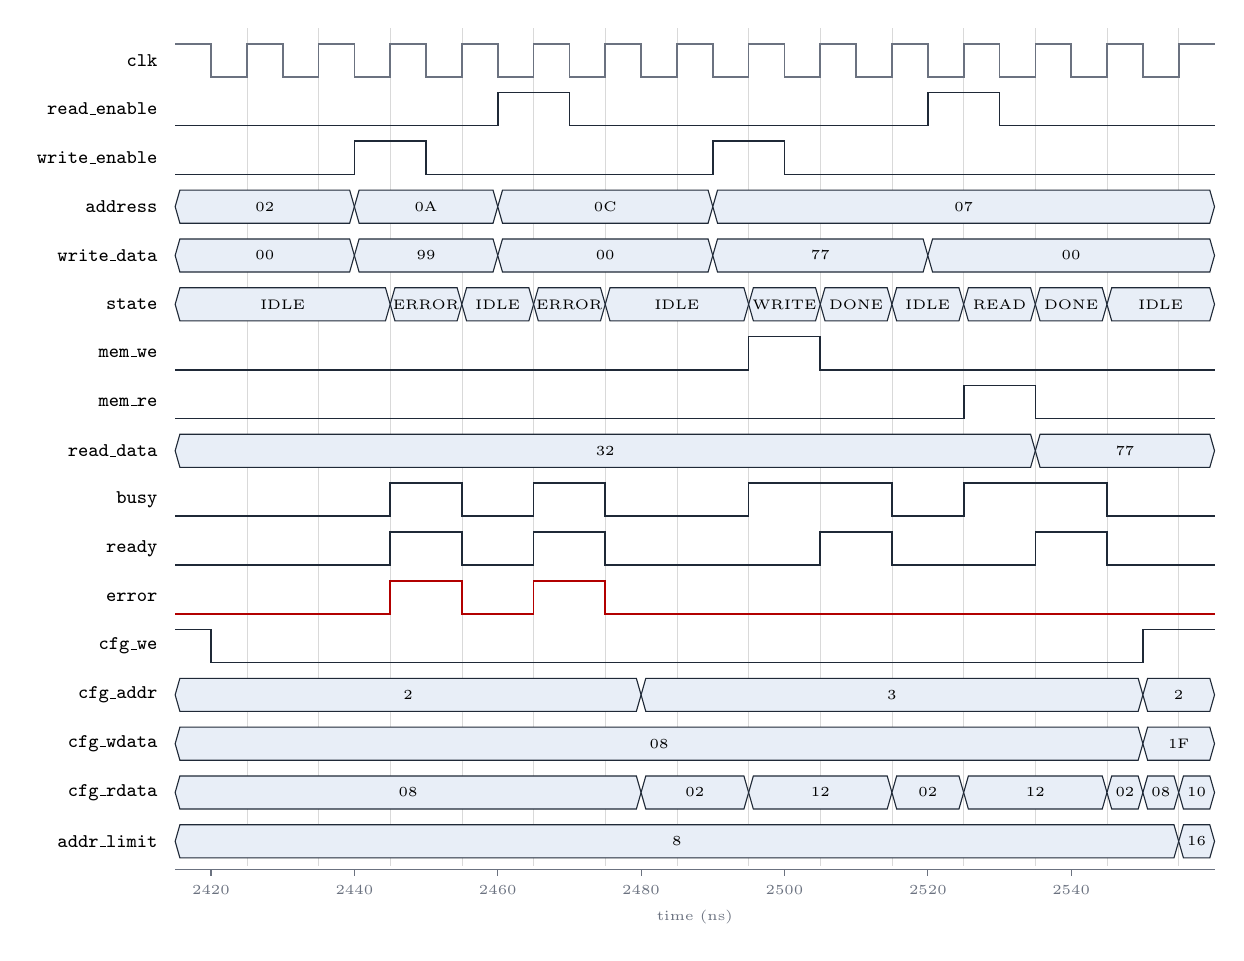
\begin{tikzpicture}[x=1cm,y=1cm,font=\scriptsize]
\draw[gray!30,very thin] (0.910,-0.1) -- (0.910,10.540);
\draw[gray!30,very thin] (1.821,-0.1) -- (1.821,10.540);
\draw[gray!30,very thin] (2.731,-0.1) -- (2.731,10.540);
\draw[gray!30,very thin] (3.641,-0.1) -- (3.641,10.540);
\draw[gray!30,very thin] (4.552,-0.1) -- (4.552,10.540);
\draw[gray!30,very thin] (5.462,-0.1) -- (5.462,10.540);
\draw[gray!30,very thin] (6.372,-0.1) -- (6.372,10.540);
\draw[gray!30,very thin] (7.283,-0.1) -- (7.283,10.540);
\draw[gray!30,very thin] (8.193,-0.1) -- (8.193,10.540);
\draw[gray!30,very thin] (9.103,-0.1) -- (9.103,10.540);
\draw[gray!30,very thin] (10.014,-0.1) -- (10.014,10.540);
\draw[gray!30,very thin] (10.924,-0.1) -- (10.924,10.540);
\draw[gray!30,very thin] (11.834,-0.1) -- (11.834,10.540);
\draw[gray!30,very thin] (12.745,-0.1) -- (12.745,10.540);
\node[anchor=east,font=\scriptsize\ttfamily] at (-0.1,10.130) {clk};
\draw[mut,line width=0.6pt] (0.000,10.340) -- (0.455,10.340) -- (0.455,9.920) -- (0.910,9.920) -- (0.910,10.340) -- (1.366,10.340) -- (1.366,9.920) -- (1.821,9.920) -- (1.821,10.340) -- (2.276,10.340) -- (2.276,9.920) -- (2.731,9.920) -- (2.731,10.340) -- (3.186,10.340) -- (3.186,9.920) -- (3.641,9.920) -- (3.641,10.340) -- (4.097,10.340) -- (4.097,9.920) -- (4.552,9.920) -- (4.552,10.340) -- (5.007,10.340) -- (5.007,9.920) -- (5.462,9.920) -- (5.462,10.340) -- (5.917,10.340) -- (5.917,9.920) -- (6.372,9.920) -- (6.372,10.340) -- (6.828,10.340) -- (6.828,9.920) -- (7.283,9.920) -- (7.283,10.340) -- (7.738,10.340) -- (7.738,9.920) -- (8.193,9.920) -- (8.193,10.340) -- (8.648,10.340) -- (8.648,9.920) -- (9.103,9.920) -- (9.103,10.340) -- (9.559,10.340) -- (9.559,9.920) -- (10.014,9.920) -- (10.014,10.340) -- (10.469,10.340) -- (10.469,9.920) -- (10.924,9.920) -- (10.924,10.340) -- (11.379,10.340) -- (11.379,9.920) -- (11.834,9.920) -- (11.834,10.340) -- (12.290,10.340) -- (12.290,9.920) -- (12.745,9.920) -- (12.745,10.340) -- (13.200,10.340);
\node[anchor=east,font=\scriptsize\ttfamily] at (-0.1,9.510) {read\_enable};
\draw[ink,line width=0.6pt] (0.000,9.300) -- (4.097,9.300) -- (4.097,9.720) -- (5.007,9.720) -- (5.007,9.300) -- (9.559,9.300) -- (9.559,9.720) -- (10.469,9.720) -- (10.469,9.300) -- (13.200,9.300);
\node[anchor=east,font=\scriptsize\ttfamily] at (-0.1,8.890) {write\_enable};
\draw[ink,line width=0.6pt] (0.000,8.680) -- (2.276,8.680) -- (2.276,9.100) -- (3.186,9.100) -- (3.186,8.680) -- (6.828,8.680) -- (6.828,9.100) -- (7.738,9.100) -- (7.738,8.680) -- (13.200,8.680);
\node[anchor=east,font=\scriptsize\ttfamily] at (-0.1,8.270) {address};
\draw[ink,fill=box,line width=0.4pt] (0.000,8.270) -- (0.060,8.060) -- (2.216,8.060) -- (2.276,8.270) -- (2.216,8.480) -- (0.060,8.480) -- cycle;
\node[font=\tiny] at (1.138,8.270) {02};
\draw[ink,fill=box,line width=0.4pt] (2.276,8.270) -- (2.336,8.060) -- (4.037,8.060) -- (4.097,8.270) -- (4.037,8.480) -- (2.336,8.480) -- cycle;
\node[font=\tiny] at (3.186,8.270) {0A};
\draw[ink,fill=box,line width=0.4pt] (4.097,8.270) -- (4.157,8.060) -- (6.768,8.060) -- (6.828,8.270) -- (6.768,8.480) -- (4.157,8.480) -- cycle;
\node[font=\tiny] at (5.462,8.270) {0C};
\draw[ink,fill=box,line width=0.4pt] (6.828,8.270) -- (6.888,8.060) -- (13.140,8.060) -- (13.200,8.270) -- (13.140,8.480) -- (6.888,8.480) -- cycle;
\node[font=\tiny] at (10.014,8.270) {07};
\node[anchor=east,font=\scriptsize\ttfamily] at (-0.1,7.650) {write\_data};
\draw[ink,fill=box,line width=0.4pt] (0.000,7.650) -- (0.060,7.440) -- (2.216,7.440) -- (2.276,7.650) -- (2.216,7.860) -- (0.060,7.860) -- cycle;
\node[font=\tiny] at (1.138,7.650) {00};
\draw[ink,fill=box,line width=0.4pt] (2.276,7.650) -- (2.336,7.440) -- (4.037,7.440) -- (4.097,7.650) -- (4.037,7.860) -- (2.336,7.860) -- cycle;
\node[font=\tiny] at (3.186,7.650) {99};
\draw[ink,fill=box,line width=0.4pt] (4.097,7.650) -- (4.157,7.440) -- (6.768,7.440) -- (6.828,7.650) -- (6.768,7.860) -- (4.157,7.860) -- cycle;
\node[font=\tiny] at (5.462,7.650) {00};
\draw[ink,fill=box,line width=0.4pt] (6.828,7.650) -- (6.888,7.440) -- (9.499,7.440) -- (9.559,7.650) -- (9.499,7.860) -- (6.888,7.860) -- cycle;
\node[font=\tiny] at (8.193,7.650) {77};
\draw[ink,fill=box,line width=0.4pt] (9.559,7.650) -- (9.619,7.440) -- (13.140,7.440) -- (13.200,7.650) -- (13.140,7.860) -- (9.619,7.860) -- cycle;
\node[font=\tiny] at (11.379,7.650) {00};
\node[anchor=east,font=\scriptsize\ttfamily] at (-0.1,7.030) {state};
\draw[ink,fill=box,line width=0.4pt] (0.000,7.030) -- (0.060,6.820) -- (2.671,6.820) -- (2.731,7.030) -- (2.671,7.240) -- (0.060,7.240) -- cycle;
\node[font=\tiny] at (1.366,7.030) {IDLE};
\draw[ink,fill=box,line width=0.4pt] (2.731,7.030) -- (2.791,6.820) -- (3.581,6.820) -- (3.641,7.030) -- (3.581,7.240) -- (2.791,7.240) -- cycle;
\node[font=\tiny] at (3.186,7.030) {ERROR};
\draw[ink,fill=box,line width=0.4pt] (3.641,7.030) -- (3.701,6.820) -- (4.492,6.820) -- (4.552,7.030) -- (4.492,7.240) -- (3.701,7.240) -- cycle;
\node[font=\tiny] at (4.097,7.030) {IDLE};
\draw[ink,fill=box,line width=0.4pt] (4.552,7.030) -- (4.612,6.820) -- (5.402,6.820) -- (5.462,7.030) -- (5.402,7.240) -- (4.612,7.240) -- cycle;
\node[font=\tiny] at (5.007,7.030) {ERROR};
\draw[ink,fill=box,line width=0.4pt] (5.462,7.030) -- (5.522,6.820) -- (7.223,6.820) -- (7.283,7.030) -- (7.223,7.240) -- (5.522,7.240) -- cycle;
\node[font=\tiny] at (6.372,7.030) {IDLE};
\draw[ink,fill=box,line width=0.4pt] (7.283,7.030) -- (7.343,6.820) -- (8.133,6.820) -- (8.193,7.030) -- (8.133,7.240) -- (7.343,7.240) -- cycle;
\node[font=\tiny] at (7.738,7.030) {WRITE};
\draw[ink,fill=box,line width=0.4pt] (8.193,7.030) -- (8.253,6.820) -- (9.043,6.820) -- (9.103,7.030) -- (9.043,7.240) -- (8.253,7.240) -- cycle;
\node[font=\tiny] at (8.648,7.030) {DONE};
\draw[ink,fill=box,line width=0.4pt] (9.103,7.030) -- (9.163,6.820) -- (9.954,6.820) -- (10.014,7.030) -- (9.954,7.240) -- (9.163,7.240) -- cycle;
\node[font=\tiny] at (9.559,7.030) {IDLE};
\draw[ink,fill=box,line width=0.4pt] (10.014,7.030) -- (10.074,6.820) -- (10.864,6.820) -- (10.924,7.030) -- (10.864,7.240) -- (10.074,7.240) -- cycle;
\node[font=\tiny] at (10.469,7.030) {READ};
\draw[ink,fill=box,line width=0.4pt] (10.924,7.030) -- (10.984,6.820) -- (11.774,6.820) -- (11.834,7.030) -- (11.774,7.240) -- (10.984,7.240) -- cycle;
\node[font=\tiny] at (11.379,7.030) {DONE};
\draw[ink,fill=box,line width=0.4pt] (11.834,7.030) -- (11.894,6.820) -- (13.140,6.820) -- (13.200,7.030) -- (13.140,7.240) -- (11.894,7.240) -- cycle;
\node[font=\tiny] at (12.517,7.030) {IDLE};
\node[anchor=east,font=\scriptsize\ttfamily] at (-0.1,6.410) {mem\_we};
\draw[ink,line width=0.6pt] (0.000,6.200) -- (7.283,6.200) -- (7.283,6.620) -- (8.193,6.620) -- (8.193,6.200) -- (13.200,6.200);
\node[anchor=east,font=\scriptsize\ttfamily] at (-0.1,5.790) {mem\_re};
\draw[ink,line width=0.6pt] (0.000,5.580) -- (10.014,5.580) -- (10.014,6.000) -- (10.924,6.000) -- (10.924,5.580) -- (13.200,5.580);
\node[anchor=east,font=\scriptsize\ttfamily] at (-0.1,5.170) {read\_data};
\draw[ink,fill=box,line width=0.4pt] (0.000,5.170) -- (0.060,4.960) -- (10.864,4.960) -- (10.924,5.170) -- (10.864,5.380) -- (0.060,5.380) -- cycle;
\node[font=\tiny] at (5.462,5.170) {32};
\draw[ink,fill=box,line width=0.4pt] (10.924,5.170) -- (10.984,4.960) -- (13.140,4.960) -- (13.200,5.170) -- (13.140,5.380) -- (10.984,5.380) -- cycle;
\node[font=\tiny] at (12.062,5.170) {77};
\node[anchor=east,font=\scriptsize\ttfamily] at (-0.1,4.550) {busy};
\draw[ink,line width=0.6pt] (0.000,4.340) -- (2.731,4.340) -- (2.731,4.760) -- (3.641,4.760) -- (3.641,4.340) -- (4.552,4.340) -- (4.552,4.760) -- (5.462,4.760) -- (5.462,4.340) -- (7.283,4.340) -- (7.283,4.760) -- (9.103,4.760) -- (9.103,4.340) -- (10.014,4.340) -- (10.014,4.760) -- (11.834,4.760) -- (11.834,4.340) -- (13.200,4.340);
\node[anchor=east,font=\scriptsize\ttfamily] at (-0.1,3.930) {ready};
\draw[ink,line width=0.6pt] (0.000,3.720) -- (2.731,3.720) -- (2.731,4.140) -- (3.641,4.140) -- (3.641,3.720) -- (4.552,3.720) -- (4.552,4.140) -- (5.462,4.140) -- (5.462,3.720) -- (8.193,3.720) -- (8.193,4.140) -- (9.103,4.140) -- (9.103,3.720) -- (10.924,3.720) -- (10.924,4.140) -- (11.834,4.140) -- (11.834,3.720) -- (13.200,3.720);
\node[anchor=east,font=\scriptsize\ttfamily] at (-0.1,3.310) {error};
\draw[red!70!black,line width=0.6pt] (0.000,3.100) -- (2.731,3.100) -- (2.731,3.520) -- (3.641,3.520) -- (3.641,3.100) -- (4.552,3.100) -- (4.552,3.520) -- (5.462,3.520) -- (5.462,3.100) -- (13.200,3.100);
\node[anchor=east,font=\scriptsize\ttfamily] at (-0.1,2.690) {cfg\_we};
\draw[ink,line width=0.6pt] (0.000,2.900) -- (0.455,2.900) -- (0.455,2.480) -- (12.290,2.480) -- (12.290,2.900) -- (13.200,2.900);
\node[anchor=east,font=\scriptsize\ttfamily] at (-0.1,2.070) {cfg\_addr};
\draw[ink,fill=box,line width=0.4pt] (0.000,2.070) -- (0.060,1.860) -- (5.857,1.860) -- (5.917,2.070) -- (5.857,2.280) -- (0.060,2.280) -- cycle;
\node[font=\tiny] at (2.959,2.070) {2};
\draw[ink,fill=box,line width=0.4pt] (5.917,2.070) -- (5.977,1.860) -- (12.230,1.860) -- (12.290,2.070) -- (12.230,2.280) -- (5.977,2.280) -- cycle;
\node[font=\tiny] at (9.103,2.070) {3};
\draw[ink,fill=box,line width=0.4pt] (12.290,2.070) -- (12.350,1.860) -- (13.140,1.860) -- (13.200,2.070) -- (13.140,2.280) -- (12.350,2.280) -- cycle;
\node[font=\tiny] at (12.745,2.070) {2};
\node[anchor=east,font=\scriptsize\ttfamily] at (-0.1,1.450) {cfg\_wdata};
\draw[ink,fill=box,line width=0.4pt] (0.000,1.450) -- (0.060,1.240) -- (12.230,1.240) -- (12.290,1.450) -- (12.230,1.660) -- (0.060,1.660) -- cycle;
\node[font=\tiny] at (6.145,1.450) {08};
\draw[ink,fill=box,line width=0.4pt] (12.290,1.450) -- (12.350,1.240) -- (13.140,1.240) -- (13.200,1.450) -- (13.140,1.660) -- (12.350,1.660) -- cycle;
\node[font=\tiny] at (12.745,1.450) {1F};
\node[anchor=east,font=\scriptsize\ttfamily] at (-0.1,0.830) {cfg\_rdata};
\draw[ink,fill=box,line width=0.4pt] (0.000,0.830) -- (0.060,0.620) -- (5.857,0.620) -- (5.917,0.830) -- (5.857,1.040) -- (0.060,1.040) -- cycle;
\node[font=\tiny] at (2.959,0.830) {08};
\draw[ink,fill=box,line width=0.4pt] (5.917,0.830) -- (5.977,0.620) -- (7.223,0.620) -- (7.283,0.830) -- (7.223,1.040) -- (5.977,1.040) -- cycle;
\node[font=\tiny] at (6.600,0.830) {02};
\draw[ink,fill=box,line width=0.4pt] (7.283,0.830) -- (7.343,0.620) -- (9.043,0.620) -- (9.103,0.830) -- (9.043,1.040) -- (7.343,1.040) -- cycle;
\node[font=\tiny] at (8.193,0.830) {12};
\draw[ink,fill=box,line width=0.4pt] (9.103,0.830) -- (9.163,0.620) -- (9.954,0.620) -- (10.014,0.830) -- (9.954,1.040) -- (9.163,1.040) -- cycle;
\node[font=\tiny] at (9.559,0.830) {02};
\draw[ink,fill=box,line width=0.4pt] (10.014,0.830) -- (10.074,0.620) -- (11.774,0.620) -- (11.834,0.830) -- (11.774,1.040) -- (10.074,1.040) -- cycle;
\node[font=\tiny] at (10.924,0.830) {12};
\draw[ink,fill=box,line width=0.4pt] (11.834,0.830) -- (11.894,0.620) -- (12.230,0.620) -- (12.290,0.830) -- (12.230,1.040) -- (11.894,1.040) -- cycle;
\node[font=\tiny] at (12.062,0.830) {02};
\draw[ink,fill=box,line width=0.4pt] (12.290,0.830) -- (12.350,0.620) -- (12.685,0.620) -- (12.745,0.830) -- (12.685,1.040) -- (12.350,1.040) -- cycle;
\node[font=\tiny] at (12.517,0.830) {08};
\draw[ink,fill=box,line width=0.4pt] (12.745,0.830) -- (12.805,0.620) -- (13.140,0.620) -- (13.200,0.830) -- (13.140,1.040) -- (12.805,1.040) -- cycle;
\node[font=\tiny] at (12.972,0.830) {10};
\node[anchor=east,font=\scriptsize\ttfamily] at (-0.1,0.210) {addr\_limit};
\draw[ink,fill=box,line width=0.4pt] (0.000,0.210) -- (0.060,0.000) -- (12.685,0.000) -- (12.745,0.210) -- (12.685,0.420) -- (0.060,0.420) -- cycle;
\node[font=\tiny] at (6.372,0.210) {8};
\draw[ink,fill=box,line width=0.4pt] (12.745,0.210) -- (12.805,0.000) -- (13.140,0.000) -- (13.200,0.210) -- (13.140,0.420) -- (12.805,0.420) -- cycle;
\node[font=\tiny] at (12.972,0.210) {16};
\draw[mut] (0,-0.15) -- (13.200,-0.15);
\draw[mut] (0.455,-0.15) -- ++(0,-0.08) node[below,font=\tiny,text=mut] {2420};
\draw[mut] (2.276,-0.15) -- ++(0,-0.08) node[below,font=\tiny,text=mut] {2440};
\draw[mut] (4.097,-0.15) -- ++(0,-0.08) node[below,font=\tiny,text=mut] {2460};
\draw[mut] (5.917,-0.15) -- ++(0,-0.08) node[below,font=\tiny,text=mut] {2480};
\draw[mut] (7.738,-0.15) -- ++(0,-0.08) node[below,font=\tiny,text=mut] {2500};
\draw[mut] (9.559,-0.15) -- ++(0,-0.08) node[below,font=\tiny,text=mut] {2520};
\draw[mut] (11.379,-0.15) -- ++(0,-0.08) node[below,font=\tiny,text=mut] {2540};
\node[font=\tiny,text=mut] at (6.600,-0.75) {time (ns)};
\end{tikzpicture}}
\caption{Address window limited to eight words}
\label{fig:range}
\end{figure}
With LIMIT = 8, the write to 0xA and the read of 0xC are rejected through ERROR. STATUS reads 0x02 (RANGE) when idle and 0x12 while a later access is in progress, because bit 4 mirrors \sig{busy}. The write and read at 0x7, the last valid word, complete normally and return 0x77. Writing 0x1F to LIMIT saturates the register to 16.

\begin{figure}[H]
\centering
\resizebox{\textwidth}{!}{%
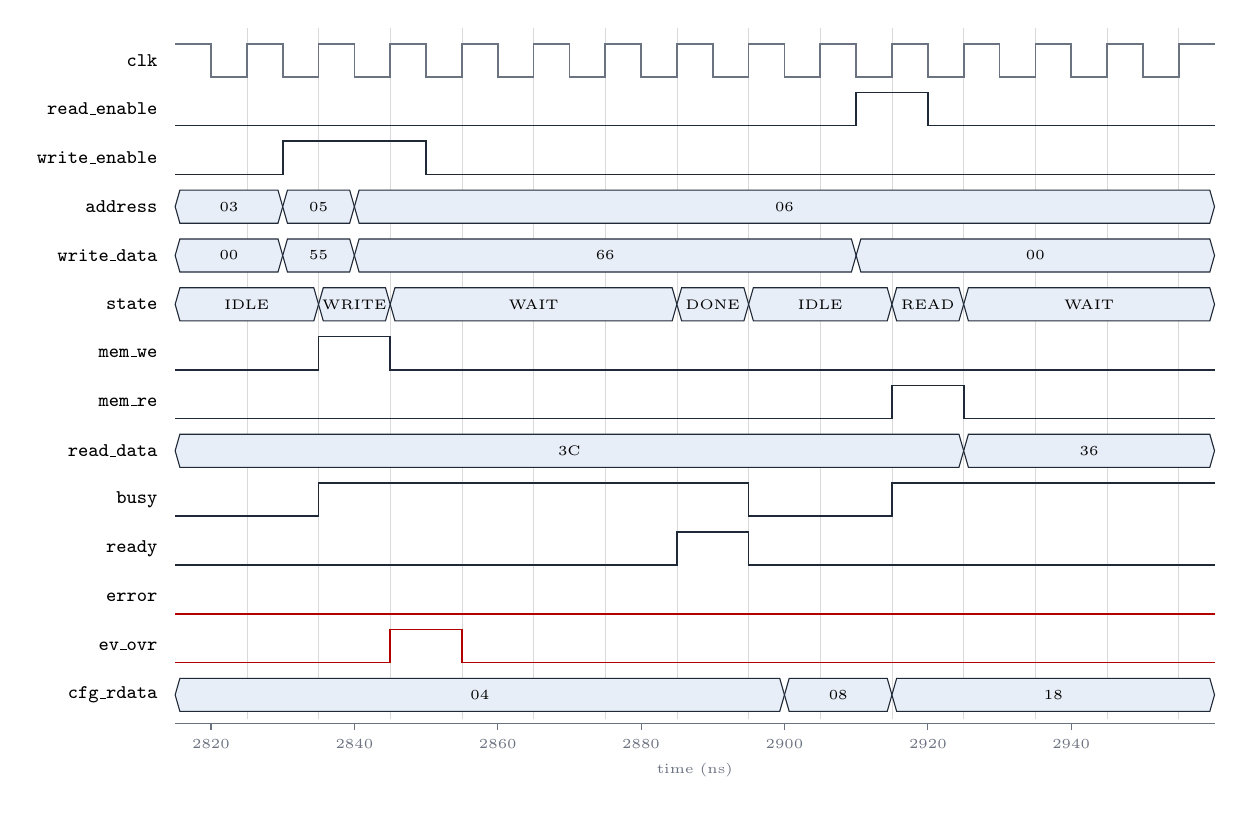
\begin{tikzpicture}[x=1cm,y=1cm,font=\scriptsize]
\draw[gray!30,very thin] (0.910,-0.1) -- (0.910,8.680);
\draw[gray!30,very thin] (1.821,-0.1) -- (1.821,8.680);
\draw[gray!30,very thin] (2.731,-0.1) -- (2.731,8.680);
\draw[gray!30,very thin] (3.641,-0.1) -- (3.641,8.680);
\draw[gray!30,very thin] (4.552,-0.1) -- (4.552,8.680);
\draw[gray!30,very thin] (5.462,-0.1) -- (5.462,8.680);
\draw[gray!30,very thin] (6.372,-0.1) -- (6.372,8.680);
\draw[gray!30,very thin] (7.283,-0.1) -- (7.283,8.680);
\draw[gray!30,very thin] (8.193,-0.1) -- (8.193,8.680);
\draw[gray!30,very thin] (9.103,-0.1) -- (9.103,8.680);
\draw[gray!30,very thin] (10.014,-0.1) -- (10.014,8.680);
\draw[gray!30,very thin] (10.924,-0.1) -- (10.924,8.680);
\draw[gray!30,very thin] (11.834,-0.1) -- (11.834,8.680);
\draw[gray!30,very thin] (12.745,-0.1) -- (12.745,8.680);
\node[anchor=east,font=\scriptsize\ttfamily] at (-0.1,8.270) {clk};
\draw[mut,line width=0.6pt] (0.000,8.480) -- (0.455,8.480) -- (0.455,8.060) -- (0.910,8.060) -- (0.910,8.480) -- (1.366,8.480) -- (1.366,8.060) -- (1.821,8.060) -- (1.821,8.480) -- (2.276,8.480) -- (2.276,8.060) -- (2.731,8.060) -- (2.731,8.480) -- (3.186,8.480) -- (3.186,8.060) -- (3.641,8.060) -- (3.641,8.480) -- (4.097,8.480) -- (4.097,8.060) -- (4.552,8.060) -- (4.552,8.480) -- (5.007,8.480) -- (5.007,8.060) -- (5.462,8.060) -- (5.462,8.480) -- (5.917,8.480) -- (5.917,8.060) -- (6.372,8.060) -- (6.372,8.480) -- (6.828,8.480) -- (6.828,8.060) -- (7.283,8.060) -- (7.283,8.480) -- (7.738,8.480) -- (7.738,8.060) -- (8.193,8.060) -- (8.193,8.480) -- (8.648,8.480) -- (8.648,8.060) -- (9.103,8.060) -- (9.103,8.480) -- (9.559,8.480) -- (9.559,8.060) -- (10.014,8.060) -- (10.014,8.480) -- (10.469,8.480) -- (10.469,8.060) -- (10.924,8.060) -- (10.924,8.480) -- (11.379,8.480) -- (11.379,8.060) -- (11.834,8.060) -- (11.834,8.480) -- (12.290,8.480) -- (12.290,8.060) -- (12.745,8.060) -- (12.745,8.480) -- (13.200,8.480);
\node[anchor=east,font=\scriptsize\ttfamily] at (-0.1,7.650) {read\_enable};
\draw[ink,line width=0.6pt] (0.000,7.440) -- (8.648,7.440) -- (8.648,7.860) -- (9.559,7.860) -- (9.559,7.440) -- (13.200,7.440);
\node[anchor=east,font=\scriptsize\ttfamily] at (-0.1,7.030) {write\_enable};
\draw[ink,line width=0.6pt] (0.000,6.820) -- (1.366,6.820) -- (1.366,7.240) -- (3.186,7.240) -- (3.186,6.820) -- (13.200,6.820);
\node[anchor=east,font=\scriptsize\ttfamily] at (-0.1,6.410) {address};
\draw[ink,fill=box,line width=0.4pt] (0.000,6.410) -- (0.060,6.200) -- (1.306,6.200) -- (1.366,6.410) -- (1.306,6.620) -- (0.060,6.620) -- cycle;
\node[font=\tiny] at (0.683,6.410) {03};
\draw[ink,fill=box,line width=0.4pt] (1.366,6.410) -- (1.426,6.200) -- (2.216,6.200) -- (2.276,6.410) -- (2.216,6.620) -- (1.426,6.620) -- cycle;
\node[font=\tiny] at (1.821,6.410) {05};
\draw[ink,fill=box,line width=0.4pt] (2.276,6.410) -- (2.336,6.200) -- (13.140,6.200) -- (13.200,6.410) -- (13.140,6.620) -- (2.336,6.620) -- cycle;
\node[font=\tiny] at (7.738,6.410) {06};
\node[anchor=east,font=\scriptsize\ttfamily] at (-0.1,5.790) {write\_data};
\draw[ink,fill=box,line width=0.4pt] (0.000,5.790) -- (0.060,5.580) -- (1.306,5.580) -- (1.366,5.790) -- (1.306,6.000) -- (0.060,6.000) -- cycle;
\node[font=\tiny] at (0.683,5.790) {00};
\draw[ink,fill=box,line width=0.4pt] (1.366,5.790) -- (1.426,5.580) -- (2.216,5.580) -- (2.276,5.790) -- (2.216,6.000) -- (1.426,6.000) -- cycle;
\node[font=\tiny] at (1.821,5.790) {55};
\draw[ink,fill=box,line width=0.4pt] (2.276,5.790) -- (2.336,5.580) -- (8.588,5.580) -- (8.648,5.790) -- (8.588,6.000) -- (2.336,6.000) -- cycle;
\node[font=\tiny] at (5.462,5.790) {66};
\draw[ink,fill=box,line width=0.4pt] (8.648,5.790) -- (8.708,5.580) -- (13.140,5.580) -- (13.200,5.790) -- (13.140,6.000) -- (8.708,6.000) -- cycle;
\node[font=\tiny] at (10.924,5.790) {00};
\node[anchor=east,font=\scriptsize\ttfamily] at (-0.1,5.170) {state};
\draw[ink,fill=box,line width=0.4pt] (0.000,5.170) -- (0.060,4.960) -- (1.761,4.960) -- (1.821,5.170) -- (1.761,5.380) -- (0.060,5.380) -- cycle;
\node[font=\tiny] at (0.910,5.170) {IDLE};
\draw[ink,fill=box,line width=0.4pt] (1.821,5.170) -- (1.881,4.960) -- (2.671,4.960) -- (2.731,5.170) -- (2.671,5.380) -- (1.881,5.380) -- cycle;
\node[font=\tiny] at (2.276,5.170) {WRITE};
\draw[ink,fill=box,line width=0.4pt] (2.731,5.170) -- (2.791,4.960) -- (6.312,4.960) -- (6.372,5.170) -- (6.312,5.380) -- (2.791,5.380) -- cycle;
\node[font=\tiny] at (4.552,5.170) {WAIT};
\draw[ink,fill=box,line width=0.4pt] (6.372,5.170) -- (6.432,4.960) -- (7.223,4.960) -- (7.283,5.170) -- (7.223,5.380) -- (6.432,5.380) -- cycle;
\node[font=\tiny] at (6.828,5.170) {DONE};
\draw[ink,fill=box,line width=0.4pt] (7.283,5.170) -- (7.343,4.960) -- (9.043,4.960) -- (9.103,5.170) -- (9.043,5.380) -- (7.343,5.380) -- cycle;
\node[font=\tiny] at (8.193,5.170) {IDLE};
\draw[ink,fill=box,line width=0.4pt] (9.103,5.170) -- (9.163,4.960) -- (9.954,4.960) -- (10.014,5.170) -- (9.954,5.380) -- (9.163,5.380) -- cycle;
\node[font=\tiny] at (9.559,5.170) {READ};
\draw[ink,fill=box,line width=0.4pt] (10.014,5.170) -- (10.074,4.960) -- (13.140,4.960) -- (13.200,5.170) -- (13.140,5.380) -- (10.074,5.380) -- cycle;
\node[font=\tiny] at (11.607,5.170) {WAIT};
\node[anchor=east,font=\scriptsize\ttfamily] at (-0.1,4.550) {mem\_we};
\draw[ink,line width=0.6pt] (0.000,4.340) -- (1.821,4.340) -- (1.821,4.760) -- (2.731,4.760) -- (2.731,4.340) -- (13.200,4.340);
\node[anchor=east,font=\scriptsize\ttfamily] at (-0.1,3.930) {mem\_re};
\draw[ink,line width=0.6pt] (0.000,3.720) -- (9.103,3.720) -- (9.103,4.140) -- (10.014,4.140) -- (10.014,3.720) -- (13.200,3.720);
\node[anchor=east,font=\scriptsize\ttfamily] at (-0.1,3.310) {read\_data};
\draw[ink,fill=box,line width=0.4pt] (0.000,3.310) -- (0.060,3.100) -- (9.954,3.100) -- (10.014,3.310) -- (9.954,3.520) -- (0.060,3.520) -- cycle;
\node[font=\tiny] at (5.007,3.310) {3C};
\draw[ink,fill=box,line width=0.4pt] (10.014,3.310) -- (10.074,3.100) -- (13.140,3.100) -- (13.200,3.310) -- (13.140,3.520) -- (10.074,3.520) -- cycle;
\node[font=\tiny] at (11.607,3.310) {36};
\node[anchor=east,font=\scriptsize\ttfamily] at (-0.1,2.690) {busy};
\draw[ink,line width=0.6pt] (0.000,2.480) -- (1.821,2.480) -- (1.821,2.900) -- (7.283,2.900) -- (7.283,2.480) -- (9.103,2.480) -- (9.103,2.900) -- (13.200,2.900);
\node[anchor=east,font=\scriptsize\ttfamily] at (-0.1,2.070) {ready};
\draw[ink,line width=0.6pt] (0.000,1.860) -- (6.372,1.860) -- (6.372,2.280) -- (7.283,2.280) -- (7.283,1.860) -- (13.200,1.860);
\node[anchor=east,font=\scriptsize\ttfamily] at (-0.1,1.450) {error};
\draw[red!70!black,line width=0.6pt] (0.000,1.240) -- (13.200,1.240);
\node[anchor=east,font=\scriptsize\ttfamily] at (-0.1,0.830) {ev\_ovr};
\draw[red!70!black,line width=0.6pt] (0.000,0.620) -- (2.731,0.620) -- (2.731,1.040) -- (3.641,1.040) -- (3.641,0.620) -- (13.200,0.620);
\node[anchor=east,font=\scriptsize\ttfamily] at (-0.1,0.210) {cfg\_rdata};
\draw[ink,fill=box,line width=0.4pt] (0.000,0.210) -- (0.060,0.000) -- (7.678,0.000) -- (7.738,0.210) -- (7.678,0.420) -- (0.060,0.420) -- cycle;
\node[font=\tiny] at (3.869,0.210) {04};
\draw[ink,fill=box,line width=0.4pt] (7.738,0.210) -- (7.798,0.000) -- (9.043,0.000) -- (9.103,0.210) -- (9.043,0.420) -- (7.798,0.420) -- cycle;
\node[font=\tiny] at (8.421,0.210) {08};
\draw[ink,fill=box,line width=0.4pt] (9.103,0.210) -- (9.163,0.000) -- (13.140,0.000) -- (13.200,0.210) -- (13.140,0.420) -- (9.163,0.420) -- cycle;
\node[font=\tiny] at (11.152,0.210) {18};
\draw[mut] (0,-0.15) -- (13.200,-0.15);
\draw[mut] (0.455,-0.15) -- ++(0,-0.08) node[below,font=\tiny,text=mut] {2820};
\draw[mut] (2.276,-0.15) -- ++(0,-0.08) node[below,font=\tiny,text=mut] {2840};
\draw[mut] (4.097,-0.15) -- ++(0,-0.08) node[below,font=\tiny,text=mut] {2860};
\draw[mut] (5.917,-0.15) -- ++(0,-0.08) node[below,font=\tiny,text=mut] {2880};
\draw[mut] (7.738,-0.15) -- ++(0,-0.08) node[below,font=\tiny,text=mut] {2900};
\draw[mut] (9.559,-0.15) -- ++(0,-0.08) node[below,font=\tiny,text=mut] {2920};
\draw[mut] (11.379,-0.15) -- ++(0,-0.08) node[below,font=\tiny,text=mut] {2940};
\node[font=\tiny,text=mut] at (6.600,-0.75) {time (ns)};
\end{tikzpicture}}
\caption{Request arriving while the controller is busy}
\label{fig:ovr}
\end{figure}
A write to 0x5 is accepted; one cycle later a write to 0x6 arrives while \sig{busy} is high. It is not latched, \sig{ev\_ovr} pulses, and STATUS reads 0x08 (OVR) once the controller is idle. The subsequent reads show that 0x5 holds 0x55 and 0x6 was not written.

\begin{figure}[H]
\centering
\resizebox{\textwidth}{!}{%
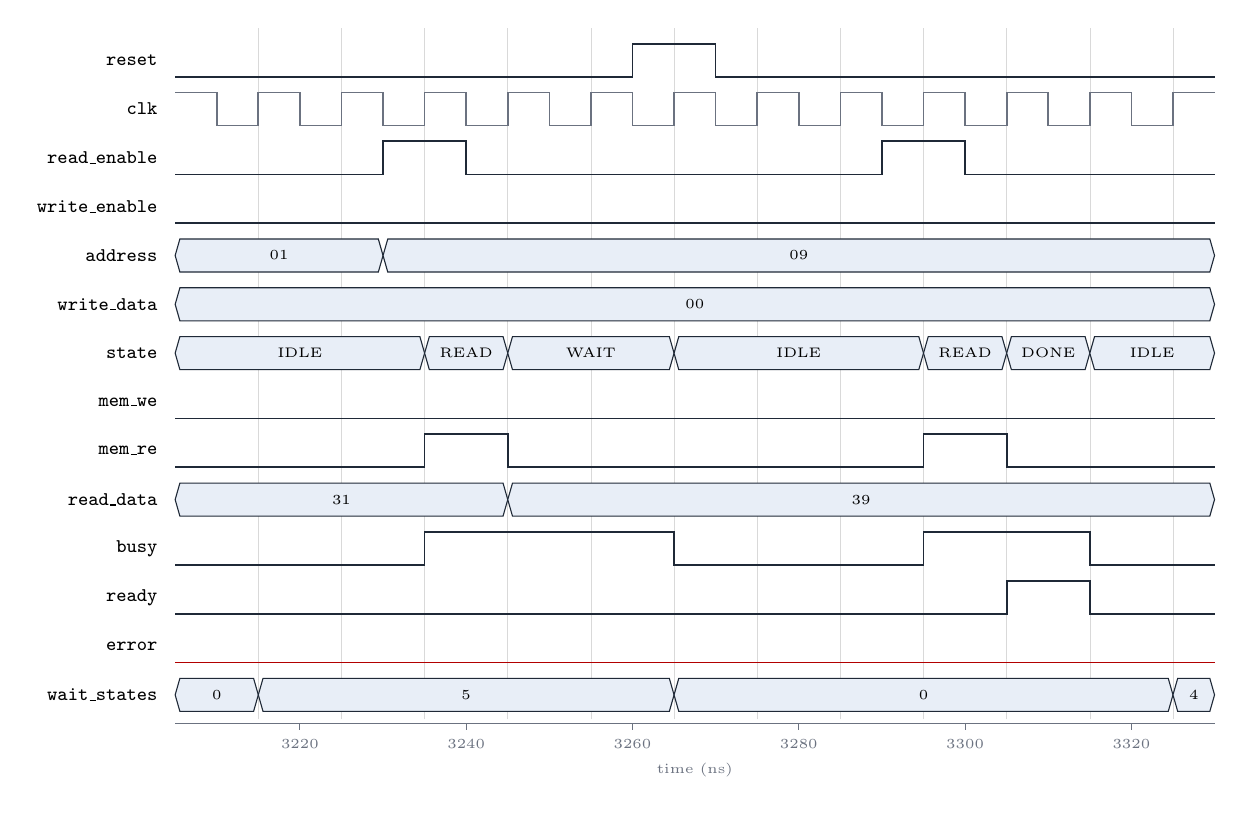
\begin{tikzpicture}[x=1cm,y=1cm,font=\scriptsize]
\draw[gray!30,very thin] (1.056,-0.1) -- (1.056,8.680);
\draw[gray!30,very thin] (2.112,-0.1) -- (2.112,8.680);
\draw[gray!30,very thin] (3.168,-0.1) -- (3.168,8.680);
\draw[gray!30,very thin] (4.224,-0.1) -- (4.224,8.680);
\draw[gray!30,very thin] (5.280,-0.1) -- (5.280,8.680);
\draw[gray!30,very thin] (6.336,-0.1) -- (6.336,8.680);
\draw[gray!30,very thin] (7.392,-0.1) -- (7.392,8.680);
\draw[gray!30,very thin] (8.448,-0.1) -- (8.448,8.680);
\draw[gray!30,very thin] (9.504,-0.1) -- (9.504,8.680);
\draw[gray!30,very thin] (10.560,-0.1) -- (10.560,8.680);
\draw[gray!30,very thin] (11.616,-0.1) -- (11.616,8.680);
\draw[gray!30,very thin] (12.672,-0.1) -- (12.672,8.680);
\node[anchor=east,font=\scriptsize\ttfamily] at (-0.1,8.270) {reset};
\draw[ink,line width=0.6pt] (0.000,8.060) -- (5.808,8.060) -- (5.808,8.480) -- (6.864,8.480) -- (6.864,8.060) -- (13.200,8.060);
\node[anchor=east,font=\scriptsize\ttfamily] at (-0.1,7.650) {clk};
\draw[mut,line width=0.6pt] (0.000,7.860) -- (0.528,7.860) -- (0.528,7.440) -- (1.056,7.440) -- (1.056,7.860) -- (1.584,7.860) -- (1.584,7.440) -- (2.112,7.440) -- (2.112,7.860) -- (2.640,7.860) -- (2.640,7.440) -- (3.168,7.440) -- (3.168,7.860) -- (3.696,7.860) -- (3.696,7.440) -- (4.224,7.440) -- (4.224,7.860) -- (4.752,7.860) -- (4.752,7.440) -- (5.280,7.440) -- (5.280,7.860) -- (5.808,7.860) -- (5.808,7.440) -- (6.336,7.440) -- (6.336,7.860) -- (6.864,7.860) -- (6.864,7.440) -- (7.392,7.440) -- (7.392,7.860) -- (7.920,7.860) -- (7.920,7.440) -- (8.448,7.440) -- (8.448,7.860) -- (8.976,7.860) -- (8.976,7.440) -- (9.504,7.440) -- (9.504,7.860) -- (10.032,7.860) -- (10.032,7.440) -- (10.560,7.440) -- (10.560,7.860) -- (11.088,7.860) -- (11.088,7.440) -- (11.616,7.440) -- (11.616,7.860) -- (12.144,7.860) -- (12.144,7.440) -- (12.672,7.440) -- (12.672,7.860) -- (13.200,7.860);
\node[anchor=east,font=\scriptsize\ttfamily] at (-0.1,7.030) {read\_enable};
\draw[ink,line width=0.6pt] (0.000,6.820) -- (2.640,6.820) -- (2.640,7.240) -- (3.696,7.240) -- (3.696,6.820) -- (8.976,6.820) -- (8.976,7.240) -- (10.032,7.240) -- (10.032,6.820) -- (13.200,6.820);
\node[anchor=east,font=\scriptsize\ttfamily] at (-0.1,6.410) {write\_enable};
\draw[ink,line width=0.6pt] (0.000,6.200) -- (13.200,6.200);
\node[anchor=east,font=\scriptsize\ttfamily] at (-0.1,5.790) {address};
\draw[ink,fill=box,line width=0.4pt] (0.000,5.790) -- (0.060,5.580) -- (2.580,5.580) -- (2.640,5.790) -- (2.580,6.000) -- (0.060,6.000) -- cycle;
\node[font=\tiny] at (1.320,5.790) {01};
\draw[ink,fill=box,line width=0.4pt] (2.640,5.790) -- (2.700,5.580) -- (13.140,5.580) -- (13.200,5.790) -- (13.140,6.000) -- (2.700,6.000) -- cycle;
\node[font=\tiny] at (7.920,5.790) {09};
\node[anchor=east,font=\scriptsize\ttfamily] at (-0.1,5.170) {write\_data};
\draw[ink,fill=box,line width=0.4pt] (0.000,5.170) -- (0.060,4.960) -- (13.140,4.960) -- (13.200,5.170) -- (13.140,5.380) -- (0.060,5.380) -- cycle;
\node[font=\tiny] at (6.600,5.170) {00};
\node[anchor=east,font=\scriptsize\ttfamily] at (-0.1,4.550) {state};
\draw[ink,fill=box,line width=0.4pt] (0.000,4.550) -- (0.060,4.340) -- (3.108,4.340) -- (3.168,4.550) -- (3.108,4.760) -- (0.060,4.760) -- cycle;
\node[font=\tiny] at (1.584,4.550) {IDLE};
\draw[ink,fill=box,line width=0.4pt] (3.168,4.550) -- (3.228,4.340) -- (4.164,4.340) -- (4.224,4.550) -- (4.164,4.760) -- (3.228,4.760) -- cycle;
\node[font=\tiny] at (3.696,4.550) {READ};
\draw[ink,fill=box,line width=0.4pt] (4.224,4.550) -- (4.284,4.340) -- (6.276,4.340) -- (6.336,4.550) -- (6.276,4.760) -- (4.284,4.760) -- cycle;
\node[font=\tiny] at (5.280,4.550) {WAIT};
\draw[ink,fill=box,line width=0.4pt] (6.336,4.550) -- (6.396,4.340) -- (9.444,4.340) -- (9.504,4.550) -- (9.444,4.760) -- (6.396,4.760) -- cycle;
\node[font=\tiny] at (7.920,4.550) {IDLE};
\draw[ink,fill=box,line width=0.4pt] (9.504,4.550) -- (9.564,4.340) -- (10.500,4.340) -- (10.560,4.550) -- (10.500,4.760) -- (9.564,4.760) -- cycle;
\node[font=\tiny] at (10.032,4.550) {READ};
\draw[ink,fill=box,line width=0.4pt] (10.560,4.550) -- (10.620,4.340) -- (11.556,4.340) -- (11.616,4.550) -- (11.556,4.760) -- (10.620,4.760) -- cycle;
\node[font=\tiny] at (11.088,4.550) {DONE};
\draw[ink,fill=box,line width=0.4pt] (11.616,4.550) -- (11.676,4.340) -- (13.140,4.340) -- (13.200,4.550) -- (13.140,4.760) -- (11.676,4.760) -- cycle;
\node[font=\tiny] at (12.408,4.550) {IDLE};
\node[anchor=east,font=\scriptsize\ttfamily] at (-0.1,3.930) {mem\_we};
\draw[ink,line width=0.6pt] (0.000,3.720) -- (13.200,3.720);
\node[anchor=east,font=\scriptsize\ttfamily] at (-0.1,3.310) {mem\_re};
\draw[ink,line width=0.6pt] (0.000,3.100) -- (3.168,3.100) -- (3.168,3.520) -- (4.224,3.520) -- (4.224,3.100) -- (9.504,3.100) -- (9.504,3.520) -- (10.560,3.520) -- (10.560,3.100) -- (13.200,3.100);
\node[anchor=east,font=\scriptsize\ttfamily] at (-0.1,2.690) {read\_data};
\draw[ink,fill=box,line width=0.4pt] (0.000,2.690) -- (0.060,2.480) -- (4.164,2.480) -- (4.224,2.690) -- (4.164,2.900) -- (0.060,2.900) -- cycle;
\node[font=\tiny] at (2.112,2.690) {31};
\draw[ink,fill=box,line width=0.4pt] (4.224,2.690) -- (4.284,2.480) -- (13.140,2.480) -- (13.200,2.690) -- (13.140,2.900) -- (4.284,2.900) -- cycle;
\node[font=\tiny] at (8.712,2.690) {39};
\node[anchor=east,font=\scriptsize\ttfamily] at (-0.1,2.070) {busy};
\draw[ink,line width=0.6pt] (0.000,1.860) -- (3.168,1.860) -- (3.168,2.280) -- (6.336,2.280) -- (6.336,1.860) -- (9.504,1.860) -- (9.504,2.280) -- (11.616,2.280) -- (11.616,1.860) -- (13.200,1.860);
\node[anchor=east,font=\scriptsize\ttfamily] at (-0.1,1.450) {ready};
\draw[ink,line width=0.6pt] (0.000,1.240) -- (10.560,1.240) -- (10.560,1.660) -- (11.616,1.660) -- (11.616,1.240) -- (13.200,1.240);
\node[anchor=east,font=\scriptsize\ttfamily] at (-0.1,0.830) {error};
\draw[red!70!black,line width=0.6pt] (0.000,0.620) -- (13.200,0.620);
\node[anchor=east,font=\scriptsize\ttfamily] at (-0.1,0.210) {wait\_states};
\draw[ink,fill=box,line width=0.4pt] (0.000,0.210) -- (0.060,0.000) -- (0.996,0.000) -- (1.056,0.210) -- (0.996,0.420) -- (0.060,0.420) -- cycle;
\node[font=\tiny] at (0.528,0.210) {0};
\draw[ink,fill=box,line width=0.4pt] (1.056,0.210) -- (1.116,0.000) -- (6.276,0.000) -- (6.336,0.210) -- (6.276,0.420) -- (1.116,0.420) -- cycle;
\node[font=\tiny] at (3.696,0.210) {5};
\draw[ink,fill=box,line width=0.4pt] (6.336,0.210) -- (6.396,0.000) -- (12.612,0.000) -- (12.672,0.210) -- (12.612,0.420) -- (6.396,0.420) -- cycle;
\node[font=\tiny] at (9.504,0.210) {0};
\draw[ink,fill=box,line width=0.4pt] (12.672,0.210) -- (12.732,0.000) -- (13.140,0.000) -- (13.200,0.210) -- (13.140,0.420) -- (12.732,0.420) -- cycle;
\node[font=\tiny] at (12.936,0.210) {4};
\draw[mut] (0,-0.15) -- (13.200,-0.15);
\draw[mut] (1.584,-0.15) -- ++(0,-0.08) node[below,font=\tiny,text=mut] {3220};
\draw[mut] (3.696,-0.15) -- ++(0,-0.08) node[below,font=\tiny,text=mut] {3240};
\draw[mut] (5.808,-0.15) -- ++(0,-0.08) node[below,font=\tiny,text=mut] {3260};
\draw[mut] (7.920,-0.15) -- ++(0,-0.08) node[below,font=\tiny,text=mut] {3280};
\draw[mut] (10.032,-0.15) -- ++(0,-0.08) node[below,font=\tiny,text=mut] {3300};
\draw[mut] (12.144,-0.15) -- ++(0,-0.08) node[below,font=\tiny,text=mut] {3320};
\node[font=\tiny,text=mut] at (6.600,-0.75) {time (ns)};
\end{tikzpicture}}
\caption{Synchronous reset applied in the middle of a read}
\label{fig:rst}
\end{figure}
Reset is asserted while the FSM is in WAIT during a five-wait-state read. On the next edge the FSM returns to IDLE, \sig{busy} falls and WAIT reverts to 0. A read of the same address afterwards returns the stored value, showing that the memory array survives a controller reset.

\subsection{Important Signal Explanations}
\begin{table}[H]
\centering
\caption{Signals shown in the waveforms}
\label{tab:sigexp}
\small
\begin{tabularx}{\textwidth}{@{}l X@{}}
\toprule
\textbf{Signal} & \textbf{Meaning in the waveforms} \\
\midrule
\sig{state} & FSM state register, decoded to state names \\
\sig{mem\_we} / \sig{mem\_re} & Internal memory strobes; exactly one cycle wide per accepted access, never asserted for a rejected one \\
\sig{busy} & High from the cycle after a request is accepted until the FSM re-enters IDLE \\
\sig{ready} & One-cycle completion pulse in DONE or ERROR \\
\sig{error} & One-cycle rejection pulse, always together with \sig{ready} \\
\sig{wcnt} & Wait-state down-counter, loaded with WAIT $-$ 1 when leaving READ or WRITE \\
\sig{ev\_ovr} & Internal pulse that sets STATUS.OVR when a request arrives while busy \\
\sig{cfg\_rdata} & Combinational read-back of the register selected by \sig{cfg\_addr} \\
\sig{addr\_limit} & Current LIMIT register value (decimal) \\
\bottomrule
\end{tabularx}
\end{table}

\subsection{Verification Summary}
\begin{table}[H]
\centering
\caption{Evidence that every specified function has been verified}
\label{tab:cov}
\small
\begin{tabularx}{\textwidth}{@{}l l X@{}}
\toprule
\textbf{Requirement} & \textbf{Tests} & \textbf{Evidence} \\
\midrule
R1 Read requests & T2, T3, T10 & 295 reads checked against model; Fig.~\ref{fig:r0} \\
R2 Write requests & T2, T3, T10 & 281 accepted writes; Fig.~\ref{fig:w0} \\
R3 Memory control signals & T2 to T7 & One-cycle strobes; none on rejection; Figs.~\ref{fig:w0}, \ref{fig:coll} \\
R4 Read data & T2, T3, T10 & Data valid with \sig{ready}; Fig.~\ref{fig:w3} \\
R5 BUSY / READY & All & busy checked every cycle of every access \\
R6 Simultaneous requests & T4 & Fig.~\ref{fig:coll} \\
R7 Invalid requests & T5, T6, T7 & Figs.~\ref{fig:range}, \ref{fig:ovr} \\
R8 Programmability & T1, T3, T5, T6, T8 & Latency 2 + WAIT for WAIT = 0 to 7; LIMIT, WP and EN behaviour \\
R9 Register-array memory & T2, T9, T10 & All 16 words; contents kept across reset; Fig.~\ref{fig:rst} \\
\bottomrule
\end{tabularx}
\end{table}

%======================== 10 SYNTHESIS ========================
\section{Synthesis Results}
\label{sec:synth}
The target is the Artix-7 device xc7a35tcpg236-1 (Basys-3 board) with a 100 MHz clock constraint (\sig{vivado/mem\_ctrl.xdc}). The Vivado flow is scripted in \sig{vivado/run\_synth.tcl}, which runs \sig{synth\_design} and writes the utilization, hierarchical utilization, timing summary and critical path reports.

The figures in this section come from Yosys 0.33 with its Xilinx 7-series flow (\sig{synth\_xilinx -family xc7}), which maps to the same primitive library (LUT1 to LUT6, MUXF7/F8, CARRY4, FDRE/FDSE, RAM32M) that Vivado uses. Synthesis completed with no latches inferred, and the final \sig{check} pass reported no problems (no combinational loops, no undriven nets). The cell report is reproduced in Table~\ref{tab:yosys}.

\begin{table}[H]
\centering
\caption{Yosys \texttt{synth\_xilinx} cell report for \texttt{mem\_ctrl\_top}}
\label{tab:yosys}
\small
\begin{tabular}{@{}l r l@{}}
\toprule
\textbf{Primitive} & \textbf{Count} & \textbf{Used for} \\
\midrule
LUT2 & 21 & \\
LUT3 & 11 & \\
LUT4 & 4 & \multicolumn{1}{l}{Next-state logic, validation, decode, read-back mux} \\
LUT5 & 4 & \\
LUT6 & 19 & \\
MUXF7 / MUXF8 & 7 / 3 & Wide multiplexers in next-state and read-back logic \\
CARRY4 & 1 & Wait-counter decrement \\
RAM32M & 1 & 16 $\times$ 8 memory array as distributed RAM \\
FDRE & 42 & Registers with synchronous reset to 0 \\
FDSE & 2 & Registers with synchronous set (EN, LIMIT[4]) \\
IBUF / OBUF / BUFG & 27 / 19 / 1 & I/O buffers and global clock buffer \\
\bottomrule
\end{tabular}
\end{table}

\IfFileExists{fig/vivado_utilization.png}{%
\begin{figure}[H]
\centering
\includegraphics[width=\textwidth]{fig/vivado_utilization.png}
\caption{Vivado utilization report after synthesis}
\end{figure}}{}

%======================== 11 TIMING ========================
\section{Timing Analysis}
\label{sec:timing}
The timing target is a 10 ns period (100 MHz). Because the design is a single synchronous domain with a synchronous reset, the only paths of interest are register-to-register paths inside \sig{clk}, plus input-to-register paths from the host pins.

A longest-path analysis of the mapped netlist (counting LUT, MUXF and CARRY cells between sequential elements) gives the following:

\begin{table}[H]
\centering
\caption{Deepest logic paths in the mapped netlist}
\label{tab:paths}
\small
\begin{tabularx}{\textwidth}{@{}c l X@{}}
\toprule
\textbf{Levels} & \textbf{Endpoint} & \textbf{Path} \\
\midrule
6 & \sig{state[1:0]} & \sig{address} / LIMIT $\to$ $\geq$ compare $\to$ IDLE decision (LUT6, MUXF7, MUXF8, LUT6, MUXF7, MUXF8) \\
5 & \sig{state[2]} & same sources, one level shorter \\
4 & \sig{ev\_range}, \sig{ev\_wpv} & same comparator feeding the error-event registers \\
3 & \sig{wcnt[2]} & state and WAIT $\to$ CARRY4 decrement \\
\bottomrule
\end{tabularx}
\end{table}

The critical path is therefore the IDLE request decision: the 5-bit address-versus-LIMIT comparison combined with the collision and write-protect checks selects among four next states. A MUXF7/MUXF8 pair adds very little delay on 7-series parts, so six levels of this kind are comfortably within a 10 ns budget; a typical Artix-7 -1 LUT plus local routing costs well under 1 ns per level. The exact worst negative slack (WNS), total negative slack and achievable $f_{max} = 1/(T - \mathrm{WNS})$ are read from \sig{reports/timing\_summary.rpt} produced by \sig{run\_synth.tcl}.

\IfFileExists{fig/vivado_timing.png}{%
\begin{figure}[H]
\centering
\includegraphics[width=\textwidth]{fig/vivado_timing.png}
\caption{Vivado timing summary after synthesis}
\end{figure}}{}

\textbf{Throughput and latency.} At 100 MHz with WAIT = 0, an access completes 20 ns after the request is sampled and a new access can start every 30 ns, giving 33.3 million accesses per second. Each wait state adds 10 ns to both figures.

%======================== 12 RESOURCES ========================
\section{Resource Utilization}
\begin{table}[H]
\centering
\caption{Resource utilization on xc7a35tcpg236-1 (from the Yosys 7-series mapping)}
\label{tab:util}
\small
\begin{tabular}{@{}l r r r@{}}
\toprule
\textbf{Resource} & \textbf{Used} & \textbf{Available} & \textbf{Utilization} \\
\midrule
Slice LUTs as logic & 59 & 20800 & 0.28\% \\
Slice LUTs as distributed RAM (RAM32M) & 4 & 9600 & 0.04\% \\
Slice registers (flip-flops) & 44 & 41600 & 0.11\% \\
F7 / F8 muxes & 7 / 3 & 16300 / 8150 & $<$0.05\% \\
Bonded IOB & 46 & 106 & 43.4\% \\
BUFGCTRL & 1 & 32 & 3.1\% \\
\bottomrule
\end{tabular}
\end{table}

The 44 flip-flops account exactly for the registers in the RTL:

\begin{table}[H]
\centering
\caption{Flip-flop budget by function}
\label{tab:ff}
\small
\begin{tabular}{@{}l l r@{}}
\toprule
\textbf{Block} & \textbf{Registers} & \textbf{Bits} \\
\midrule
FSM & state (3), wcnt (3), addr\_q (4), wdata\_q (8), error events (4) & 22 \\
Configuration & EN (1), WP (1), WAIT (3), LIMIT (5), STATUS sticky bits (4) & 14 \\
Memory & registered read output \sig{mem\_rdata} & 8 \\
\midrule
\textbf{Total} & & \textbf{44} \\
\bottomrule
\end{tabular}
\end{table}

The 128 storage bits of the array do not appear as flip-flops: because the array has no reset and a single synchronous write port, it is inferred as one RAM32M distributed-RAM primitive (four LUTs used as memory). Vivado normally performs the same inference; if it instead builds the array from registers, the flip-flop count rises by 128 and the LUT count by the read multiplexer, still well below 1\% of the device. The IOB figure is high only because every port is brought to a pin for a standalone build; when the controller is embedded in a larger design these ports become internal nets.

%======================== 13 CHALLENGES ========================
\section{Design Challenges}
\begin{enumerate}[leftmargin=*,itemsep=3pt]
\item \textbf{Read-data alignment.} The memory has a registered output, so the read value appears one cycle after \sig{mem\_re}. Placing DONE directly after READ (or after WAIT) and driving \sig{read\_data} straight from the memory register makes the data valid exactly when \sig{ready} is high, without an extra holding register.
\item \textbf{Wait-state counting off-by-one.} Loading the counter with WAIT and leaving WAIT on zero produced one extra cycle. The counter is loaded with WAIT $-$ 1 when leaving READ or WRITE; the latency check in T3 (2 + WAIT for all eight settings) caught the incorrect variant during mutation testing.
\item \textbf{Defining ``simultaneous'' and ``invalid''.} The specification leaves the policy open. Rejecting a collision, rather than giving priority to one operation, was chosen because silently dropping one of two requests hides a bug in the requesting block. A fixed check order (collision, range, protection) gives each rejected request exactly one reason in STATUS.
\item \textbf{Sticky status versus clear.} An error event arriving in the same cycle as a W1C clear could be lost. The update \sig{sticky <= (sticky \& \textasciitilde clr) | set} gives the event priority.
\item \textbf{Testbench races.} Driving and sampling on the same clock edge produced order-dependent results in early runs. Driving on the falling edge and sampling half a cycle after the active edge removed the ambiguity.
\end{enumerate}

%======================== 14 IMPROVEMENTS ========================
\section{Possible Improvements}
\begin{itemize}[leftmargin=*,itemsep=3pt]
\item \textbf{Pipelined back-to-back access.} Accepting a new request in DONE (or using a one-entry request queue) would raise throughput from one access per 3 cycles to one per 2 at WAIT = 0.
\item \textbf{Shorter critical path.} Registering the address-range check (precomputing a valid flag when the address arrives) would remove the comparator from the next-state path.
\item \textbf{Burst transfers.} A burst-length register and an auto-incrementing address counter would let one request move several consecutive words.
\item \textbf{Standard bus interface.} Wrapping the request port as an AXI4-Lite or APB slave would allow direct connection to a MicroBlaze or Zynq processing system.
\item \textbf{Block RAM and error protection.} For larger depths the array can be mapped to BRAM, and a Hamming SEC-DED code can be added to detect and correct single-bit upsets.
\item \textbf{Assertion-based checks.} SystemVerilog assertions (for example, \sig{mem\_we} and \sig{mem\_re} never high together, \sig{ready} always one cycle wide) and functional coverage would strengthen verification.
\end{itemize}

%======================== 15 CONCLUSION ========================
\section{Conclusion}
A programmable synchronous memory controller for a 16 $\times$ 8 on-chip register-array memory was designed in synthesizable Verilog, verified with a self-checking testbench that passed all 3356 checks across ten test groups, and synthesized for the Artix-7 fabric using 59 LUTs, one distributed RAM primitive and 44 flip-flops with a six-level critical path well within the 100 MHz target.

\end{document}
